\section{Self-sufficient energy distribution system} \label{sec:energy}
Now the self-suficient energy distribution system of the repeater radio infrastructure is being examined. For this purpose, the PV generators used are first introduced and their behavior for different values of the PV cell temperature $\vartheta_\mathrm{C}$ and the solar irradiance $E_\mathrm{G}$ is examined based on the model mentioned in the subsection \ref{sec:photovoltaic_generators}. The $\mathrm{LiFePO}_4$ battery used is then introduced and the results from the experiments discussed in the subsection \ref{sec:electrochemical} are presented. Finally, the remaining components required for the self-sufficient energy distribution system are introduced and a performance estimation based on a \MATLAB simulation (see appendix \ref{sec:matlab_code}) is carried out in order to assess whether it can supply the repeater radio infrastructure with electrical energy. 

\subsection{Photovoltaic generator model} \label{sec:pv_gen_mod}
In general, two different PV generators are examined. Namely the AE Solar AE195SMM6-36 and the DAS Energy DAS145PF. Only one (primary) PV generator is used to suppliy the repeater radio infrastructure with electrical energy, with the second one serving as a backup. The backup PV generator is installed when the primary one fails to convert the required amount of electrical energy. This is the case, for example, if it gets damaged during an ongoing mission. Since both PV generators have a similar power output $P_\mathrm{PV}$, it is up to the OeWF to decide which one is used as the primary and which one as the backup. Excerpts from their data sheets can be found in the tables \ref{tab:table_ae_solar_pvg_specs} and \ref{tab:table_das_energy_pvg_specs}.
\begin{table}[h!]
	\centering
	\footnotesize
\begin{tabular}{|l|c|}
	\hline
	\multicolumn{2}{|c|}{\textbf{AE Solar AE195SMM6-36 specifications}} \\
	\hline
	PV cell type & 5BB Monocrystalline \\
	PV cell area & $156,75 \cdot 156,75\mathrm{mm}^2$ \\
	Number of PV cells & $36$ $(4 \cdot 9)$ \\
	Wind load & $244\mathrm{kg}\mathrm{m}^{-2}$ \\
	Mechanical load & $550\mathrm{kg}/\mathrm{m}^2$ \\
	Operating temperature & $-40^\circ \mathrm{C}$ to $85^\circ \mathrm{C}$ \\
	\hline
 	Maximum system voltage & $1000\mathrm{V}$ \\
	Maximum series fuse rating & $10\mathrm{A}$ \\
	Short-circuit current & $9,79\mathrm{A}$ \\
	Open-circuit voltage & $25,87\mathrm{V}$ \\
	MPP current & $9,11\mathrm{A}$ \\
	MPP voltage & $21,41\mathrm{V}$ \\
	Nominal MPP power & $195,0\mathrm{W}$ (peak) \\
	NOCT & $45\pm2 ^\circ \mathrm{C}$ \\
	Efficiency & $19,25\%$ \\
	\hline
	Temperature coeff. for $P_{\mathrm{MPP}}$ & $-0,380 \%^\circ \mathrm{C}^{-1}$ \\
	Temperature coeff. for $U_{\mathrm{OC}}$ & $-0,290 \%^\circ \mathrm{C}^{-1}$ \\
	Temperature coeff. for $I_{\mathrm{SC}}$ & $0,050 \%^\circ \mathrm{C}^{-1}$ \\
	\hline
\end{tabular}
	\caption{Excerpt from the data sheet of the AE Solar AE195SMM6-36 PV generator at STC \cite{ae_solar:2019}.}
	\label{tab:table_ae_solar_pvg_specs}
\end{table}
\begin{table}[h!]
	\centering
	\footnotesize
\begin{tabular}{|l|c|}
	\hline
	\multicolumn{2}{|c|}{\textbf{DAS Energy DAS145PF specifications}} \\
	\hline
	PV cell type & 3BB Polycrystalline \\
	PV cell area & $156,75 \cdot 156,75\mathrm{mm}^2$ \\
	Number of PV cells & $36$ $(4 \cdot 9)$ \\
	Operating temperature & $-40^\circ \mathrm{C}$ to $85^\circ \mathrm{C}$ \\
	\hline
 	Maximum system voltage & $1000\mathrm{V}$ \\
	Maximum series fuse rating & $20\mathrm{A}$ \\
	Short-circuit current & $8,69\mathrm{A}$ \\
	Open-circuit voltage & $22,85\mathrm{V}$ \\
	MPP current & $8,19\mathrm{A}$ \\
	MPP voltage & $18,69\mathrm{V}$ \\
	Nominal MPP power & $153,1\mathrm{W}$ (peak) \\
	\hline
	Temperature coeff. for $P_{\mathrm{MPP}}$ & $-0,393 \%^\circ \mathrm{C}^{-1}$ \\
	Temperature coeff. for $U_{\mathrm{OC}}$ & $-0,310 \%^\circ \mathrm{C}^{-1}$ \\
	Temperature coeff. for $I_{\mathrm{SC}}$ & $0,051 \%^\circ \mathrm{C}^{-1}$ \\
	\hline
\end{tabular}
	\caption{Excerpt from the data sheet of the DAS Energy DAS145PF PV generator at STC \cite{das_energy_2017}.}
	\label{tab:table_das_energy_pvg_specs}
\end{table}

As can be seen from the results of the \MAPLE source code in the appendix \ref{sec:maple_code}, it makes little difference for the first few decimal places if the model is approximated with the Jacobian matrix. In the \MAPLE source code, the caluclations are performed for the AE Solar AE195SMM6-36 PV generator, with its PV cell temperature being $\vartheta_\mathrm{C} = 25^\circ\mathrm{C}$ and the total irradiance onto its inclined surface being $E_\mathrm{G} = 200\mathrm{Wm}^{-2}$. These results can be replicated for the DAS Energy DAS145PF PV generator and for other values of $\vartheta_\mathrm{C}$ and $E_\mathrm{G}$ as well. Therefore, it can be said that the starting values shown in the equation (\ref{eq:U_OC_I_S_zero}) suffice as a good approximation for the PV generator's open-circuit voltage $U_\mathrm{OC}$ and reverse saturation current $I_\mathrm{S}$. This is because $I_\mathrm{S}$ is usually very small \cite{Mertens:2015, Wagner:2018}. 

The results for the modeled current-voltage and power-voltage characteristics of the AE Solar AE195SMM6-36 PV generator, depending on either the total irradiance onto its inclined surface $E_\mathrm{G}$ or on its PV cell temperature $\vartheta_\mathrm{C}$, can be seen in the figures \ref{fig:image_curr_volt_irr_ae_solar}, \ref{fig:image_power_volt_irr_ae_solar}, \ref{fig:image_curr_volt_temp_ae_solar} and \ref{fig:image_power_volt_temp_ae_solar}. If it depends on $E_\mathrm{G}$ it is assumed that $\vartheta_\mathrm{C} = 25^\circ\mathrm{C}$ is constant, and if it depends on $\vartheta_\mathrm{C}$ it is assumed that $E_\mathrm{G} = 1000\mathrm{Wm}^{-2}$ is constant. These constant vlaues for $\vartheta_\mathrm{C}$ and $E_\mathrm{G}$ were chosen because they represent the STCs. Identically, the results for the DAS Energy DAS145PF PV generator can be taken from the figures \ref{fig:image_curr_volt_irr_das_energy}, \ref{fig:image_power_volt_irr_das_energy}, \ref{fig:image_curr_volt_temp_das_energy} and \ref{fig:image_power_volt_temp_das_energy}. All results were obtained by programming the discussed model of a PV generator in \MATLAB.

From the current-voltage characteristics for different irradiance levels $E_\mathrm{G}$ of both PV generators shown in the figures \ref{fig:image_curr_volt_irr_ae_solar} and \ref{fig:image_curr_volt_irr_das_energy}, it can be seen that the short-circuit current $I_\mathrm{SC}$ decreases faster than the open-circuit voltage $U_\mathrm{OC}$. This is due to the fact that $I_\mathrm{Ph} = I_\mathrm{SC}$ is proportional to $E_\mathrm{G}$ (compare to equation (\ref{eq:i_ph_theta_phi})), while $U_\mathrm{OC}$ changes with the natural logarithm to it (compare to equations (\ref{eq:U_OC_theta_phi}) and \ref{eq:U_OC_I_S_zero})) \cite{Mertens:2015}.
\begin{figure}[h!]
	\centering
  	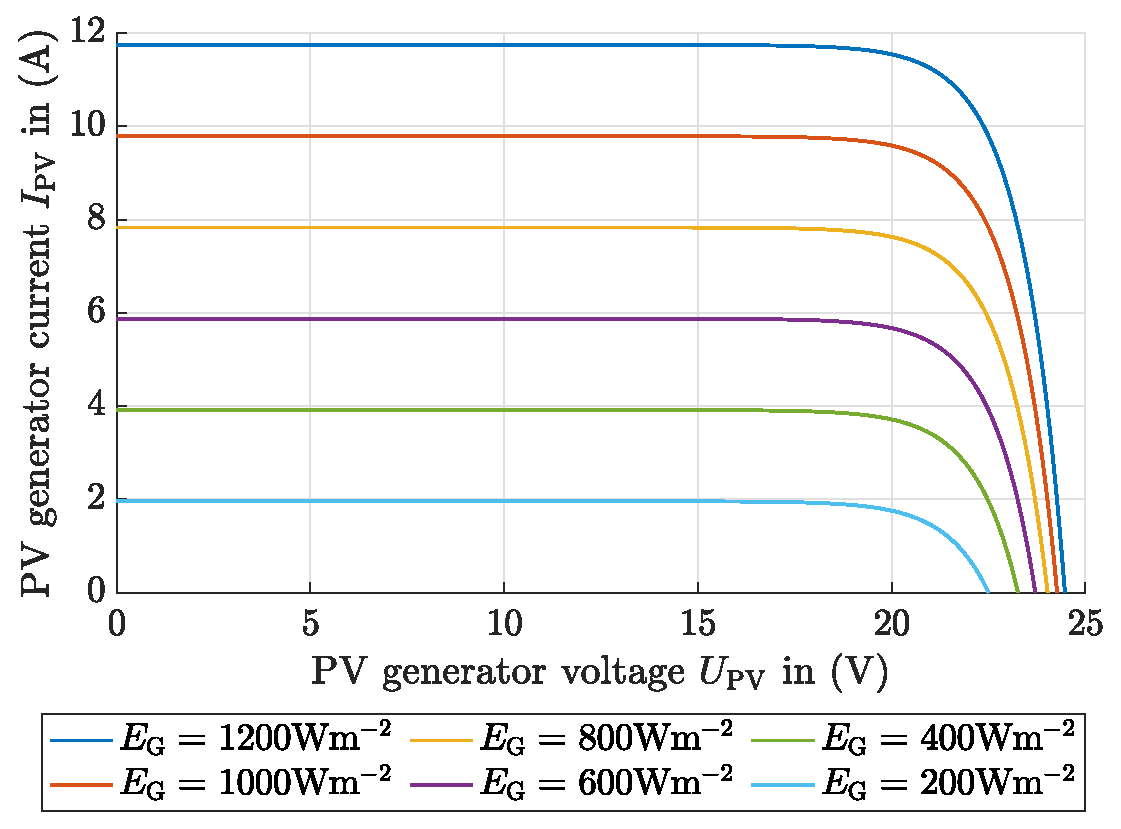
\includegraphics[width = 0.67\textwidth]{image_curr_volt_irr_ae_solar.eps}
  	\caption{Modeled current-voltage characteristic of the AE Solar AE195SMM6-36 PV generator, depending on the total irradiance onto its inclined surface $E_\mathrm{G}$. The PV cell temperature $\vartheta_\mathrm{C} = 25^\circ\mathrm{C}$ is assumed to be constant.}
	\label{fig:image_curr_volt_irr_ae_solar}
\end{figure}
\begin{figure}[h!]
	\centering
  	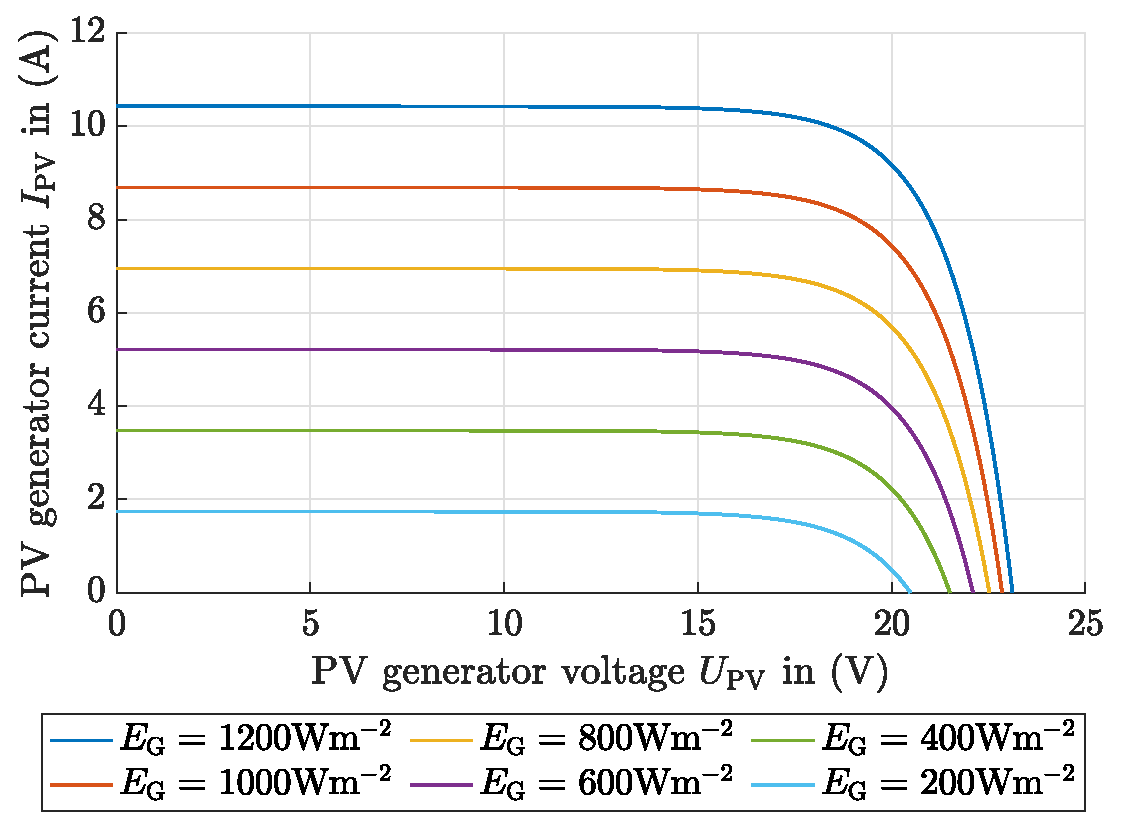
\includegraphics[width = 0.67\textwidth]{image_curr_volt_irr_das_energy.eps}
  	\caption{Modeled current-voltage characteristic of the DAS Energy DAS145PF PV generator, depending on the total irradiance onto its inclined surface $E_\mathrm{G}$. The PV cell temperature $\vartheta_\mathrm{C} = 25^\circ\mathrm{C}$ is assumed to be constant.}
	\label{fig:image_curr_volt_irr_das_energy}
\end{figure}

Now the associated power-voltage characteristics for different irradiance levels $E_\mathrm{G}$ of both PV generators can be calculated by using the equation (\ref{eq:p_pv_u}), as shown in the figures \ref{fig:image_power_volt_irr_ae_solar} and \ref{fig:image_power_volt_irr_das_energy}. As can be observed from a real PV generator, the power output $P_\mathrm{PV}$ decreases with lower irradiance levels $E_\mathrm{G}$. 
\begin{figure}[h!]
	\centering
  	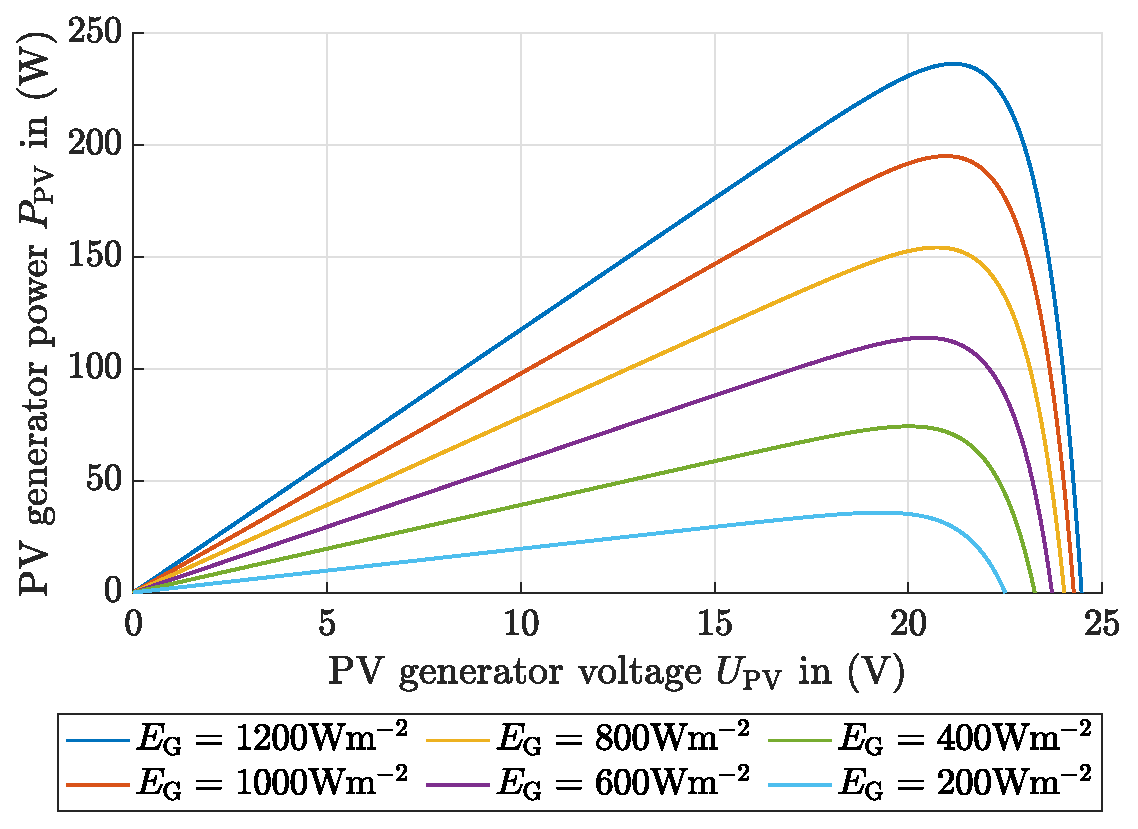
\includegraphics[width = 0.67\textwidth]{image_power_volt_irr_ae_solar.eps}
  	\caption{Modeled power-voltage characteristic of the AE Solar AE195SMM6-36 PV generator, depending on the total irradiance onto its inclined surface $E_\mathrm{G}$. The PV cell temperature $\vartheta_\mathrm{C} = 25^\circ\mathrm{C}$ is assumed to be constant.}
	\label{fig:image_power_volt_irr_ae_solar}
\end{figure}
\begin{figure}[h!]
	\centering
  	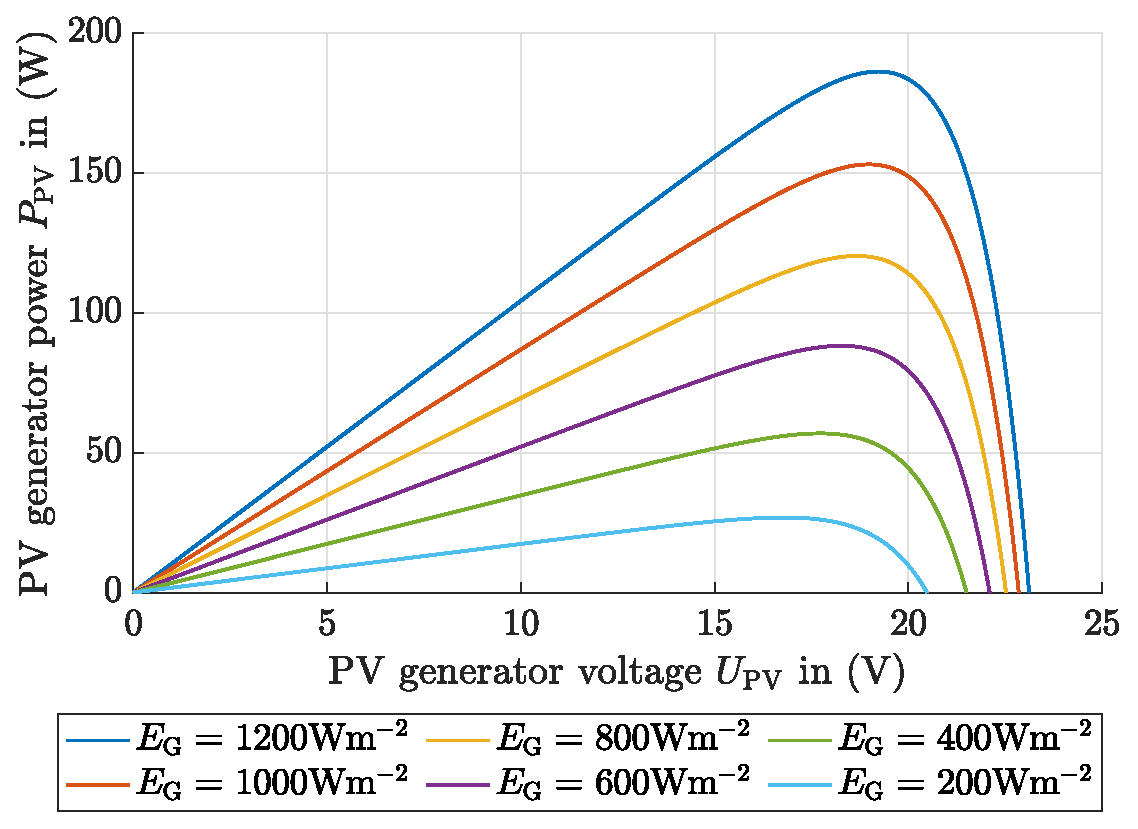
\includegraphics[width = 0.67\textwidth]{image_power_volt_irr_das_energy.eps}
  	\caption{Modeled power-voltage characteristic of the DAS Energy DAS145PF PV generator, depending on the total irradiance onto its inclined surface $E_\mathrm{G}$. The PV cell temperature $\vartheta_\mathrm{C} = 25^\circ\mathrm{C}$ is assumed to be constant.}
	\label{fig:image_power_volt_irr_das_energy}
\end{figure}

Another interesting behavior of the PV generators can be observed for different temperatures $\vartheta_\mathrm{C}$ of their PV cells. Due to the temperature increse of the semiconductors, the current $I_\mathrm{Ph} = I_\mathrm{SC}$ increses, however not as much as the voltage $U_\mathrm{OC}$ decreses. 
\begin{figure}[h!]
	\centering
  	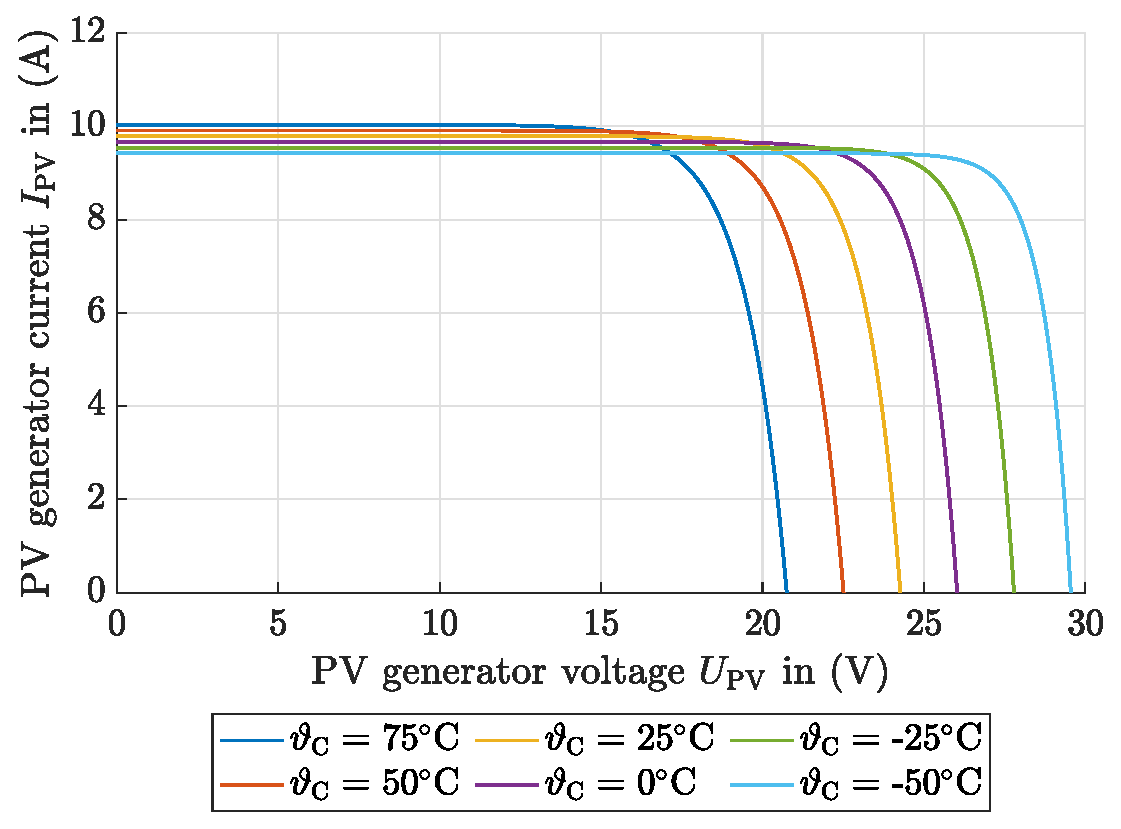
\includegraphics[width = 0.67\textwidth]{image_curr_volt_temp_ae_solar.eps}
  	\caption{Modeled current-voltage characteristic of the AE Solar AE195SMM6-36 PV generator, depending on its PV cell temperature $\vartheta_\mathrm{C}$. The total irradiance onto its inclined surface $E_\mathrm{G} = 1000\mathrm{Wm}^{-2}$ is assumed to be constant.}
	\label{fig:image_curr_volt_temp_ae_solar}
\end{figure}
\begin{figure}[h!]
	\centering
  	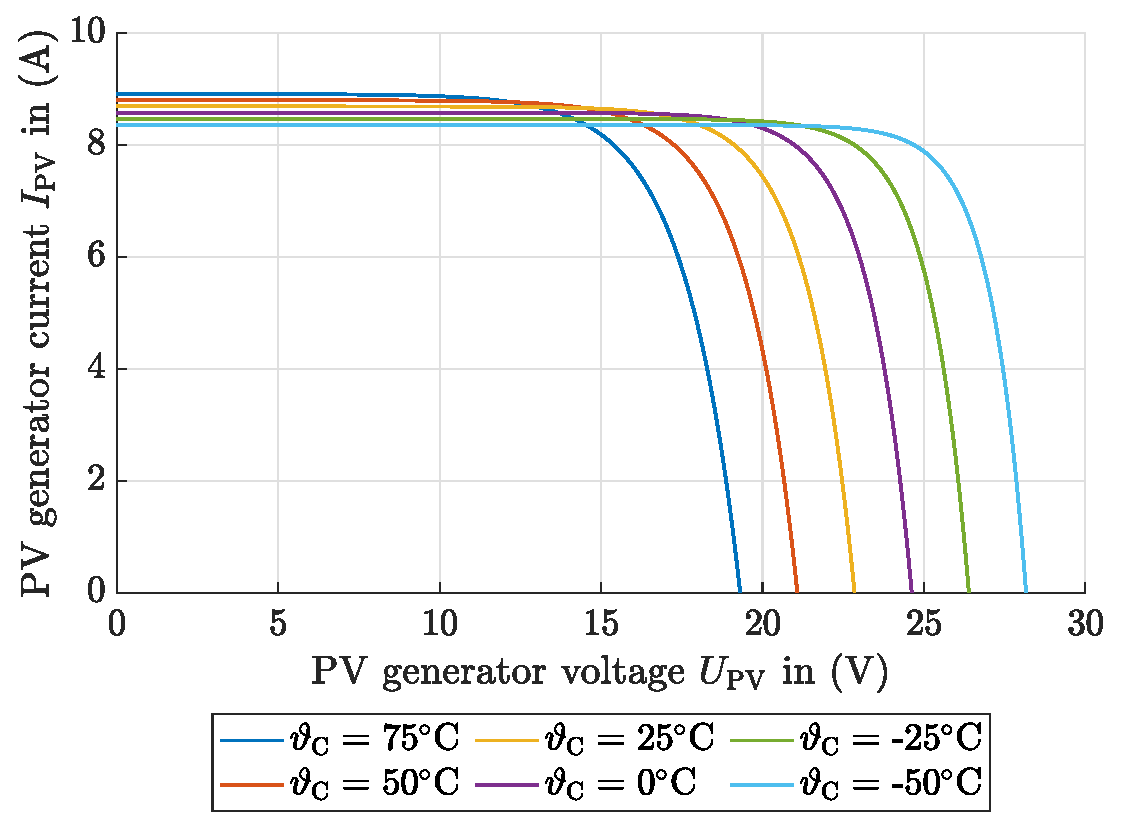
\includegraphics[width = 0.67\textwidth]{image_curr_volt_temp_das_energy.eps}
  	\caption{Modeled current-voltage characteristic of the DAS Energy DAS145PF PV generator, depending on its PV cell temperature $\vartheta_\mathrm{C}$. The total irradiance onto its inclined surface $E_\mathrm{G} = 1000\mathrm{Wm}^{-2}$ is assumed to be constant.}
	\label{fig:image_curr_volt_temp_das_energy}
\end{figure}
This finding results in an overall decrease in the power output $P_\mathrm{PV}$ of the PV generators for rising temperatures $\vartheta_\mathrm{C}$. Similarly, such behavior can be observed for decreasing temperatures $\vartheta_\mathrm{C}$. Here the overall power output $P_\mathrm{PV}$ increases. This is shown in the figures \ref{fig:image_curr_volt_temp_ae_solar} and \ref{fig:image_curr_volt_temp_das_energy}. When modeling a self-sufficient energy system, this factor must therefore not be neglected \cite{Mertens:2015}. 
\begin{figure}[h!]
	\centering
  	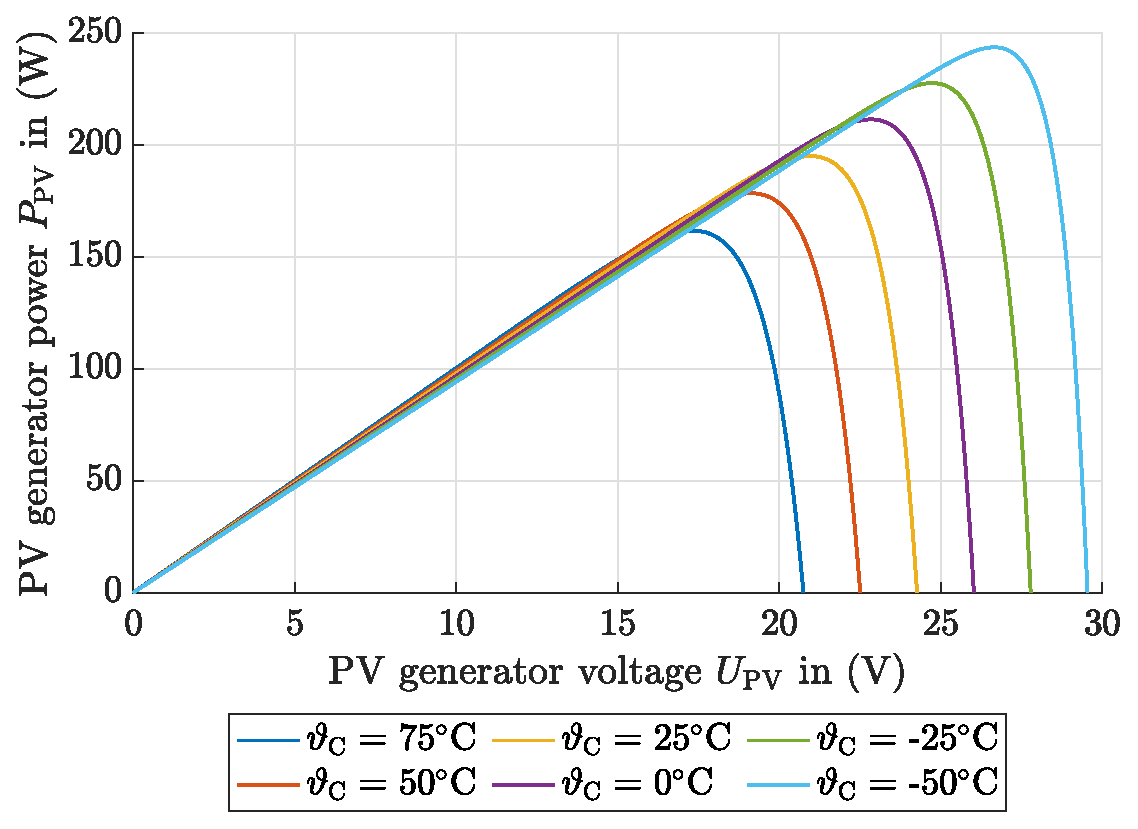
\includegraphics[width = 0.67\textwidth]{image_power_volt_temp_ae_solar.eps}
  	\caption{Modeled power-voltage characteristic of the AE Solar AE195SMM6-36 PV generator, depending on its PV cell temperature $\vartheta_\mathrm{C}$. The total irradiance onto its inclined surface $E_\mathrm{G} = 1000\mathrm{Wm}^{-2}$ is assumed to be constant.}
	\label{fig:image_power_volt_temp_ae_solar}
\end{figure}
\begin{figure}[h!]
	\centering
  	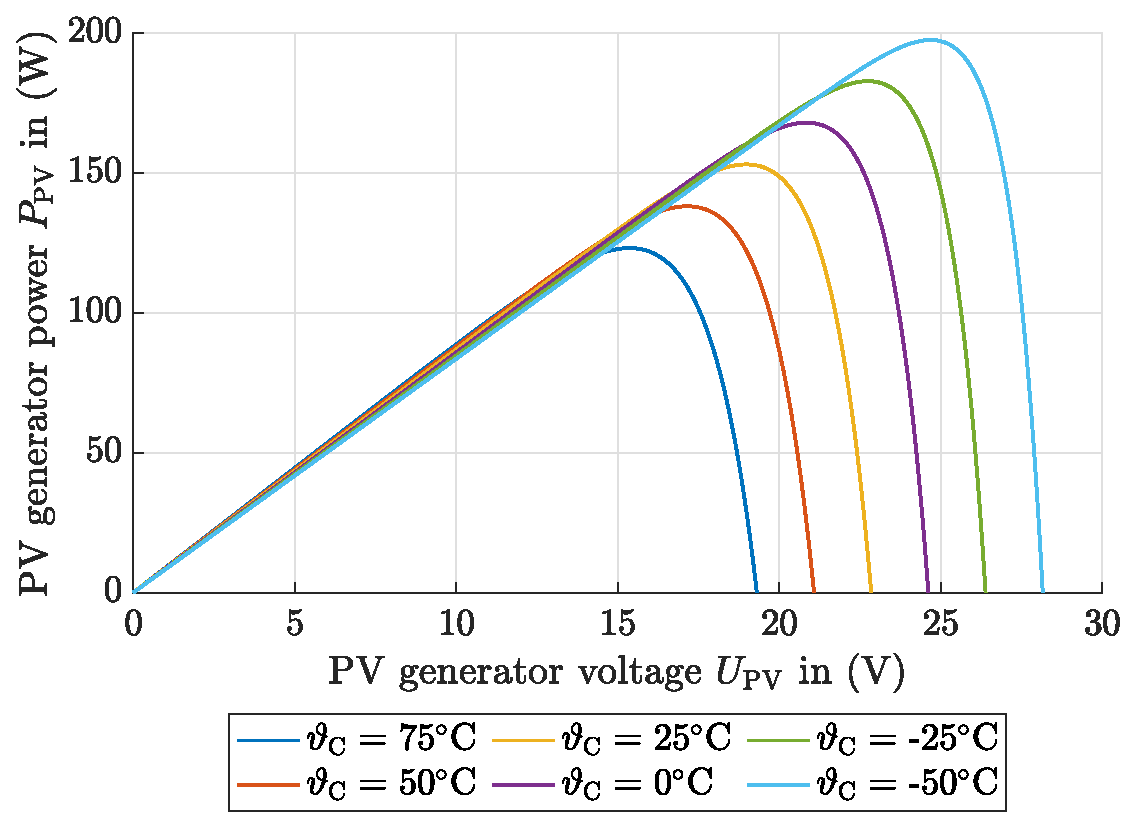
\includegraphics[width = 0.67\textwidth]{image_power_volt_temp_das_energy.eps}
  	\caption{Modeled power-voltage characteristic of the DAS Energy DAS145PF PV generator, depending on its PV cell temperature $\vartheta_\mathrm{C}$. The total irradiance onto its inclined surface $E_\mathrm{G} = 1000\mathrm{Wm}^{-2}$ is assumed to be constant.}
	\label{fig:image_power_volt_temp_das_energy}
\end{figure}

With the help of the aforementioned \MATLAB program, the ideality factors of the two PV generators were empirically determined in such a way that their power output at MPP for STCs corresponds to that in their data sheets. This resulted in an ideality factor of $m = 1,19045$ for the AE Solar AE195SMM6-36 PV generator and $m = 1,58972$ for the DAS Energy DAS145PF PV generator -- for an accuracy of two decimal places. 


 






\clearpage
\subsection{$\boldsymbol{\mathrm{LiFePO}_4}$ battery model} \label{sec_bat_res}
As already mentioned, the Offgridtec Smart-Pro $12,8\mathrm{V}$ $50\mathrm{Ah}$ $\mathrm{LiFePO_4}$ battery -- which from now on will simply be refered to as battery -- is used to store the electrical energy converted by the PV generator and to supply the repeater radio infrastructure with it. Table \ref{tab:table_smart_pro_lifepo4_battery} contains an excerpt from the data sheet for this battery, with which the nominal current of the battery can be calculated using the equation (\ref{eq:i_nom}) to $I_\mathrm{nom} = 16,67\mathrm{A}$. 
\begin{table}[h!]
	\centering
	\footnotesize
\begin{tabular}{|l|c|}
	\hline
	\multicolumn{2}{|c|}{\textbf{Offgridtec Smart-Pro $\boldsymbol{12,8\mathrm{V}}$ $\boldsymbol{50\mathrm{Ah}}$ specifications}} \\
	\hline
	Nominal charge for $\mathrm{C_D} = 1/3\mathrm{h}^{-1}$ & $50\mathrm{Ah}$ \\
	Nominal discharging current & $16,7\mathrm{A}$ \\
	Nominal voltage & $12,8\mathrm{V}$ \\
	Working voltage & $11,0\mathrm{V}$ to $14,6\mathrm{V}$ \\
	Maximum continuous discharging current & $50\mathrm{A}$ \\
	Recommended continuous discharging current & $20\mathrm{A}$ \\
	Maximum charging current & $50\mathrm{A}$ \\
	Recommended charging current & $25\mathrm{A}$ \\
	Maximum charging voltage & $14,4\pm0,2\mathrm{V}$ \\
	Float charge voltage & $13,8\pm0,2\mathrm{V}$ \\
	Minimum number of cycles & $>2500$ \\
	\hline
	Charging temperature & $-20^\circ\mathrm{C}$ to $60^\circ\mathrm{C}$ \\
	Discharging temperature & $-5^\circ\mathrm{C}$ to $45^\circ\mathrm{C}$ \\
	Storage temperature ($20\%$ to $75\%$ humidity) & $0^\circ\mathrm{C}$ to $20^\circ\mathrm{C}$ \\
	\hline
	BMS & Integrated \\
	Bluetooth & Integrated \\
	\hline
\end{tabular}
	\caption{Excerpt from the data sheet of the Offgridtec Smart-Pro $12,8\mathrm{V}$ $50\mathrm{Ah}$ $\mathrm{LiFePO_4}$ battery \cite{Offgridtec:2020}.}
	\label{tab:table_smart_pro_lifepo4_battery}
\end{table}

So that this battery can be used with the \MATLAB simulation in the appendix \ref{sec:matlab_code}, the discharging and charging experiments discussed in the subsection \ref{sec:electrochemical} had to be carried out. The laboratory equipment required for these experiments is listed in the table \ref{tab:table_dis_chrg_exp_equipm}.
\begin{table}[h!]
	\centering
	\footnotesize
\begin{tabular}{|l|c|}
	\hline
	\multicolumn{2}{|c|}{\textbf{Laboratory equipment}} \\
	\hline
	Oscilloscope & Keysight DSOX 1102G \\
	Shunt resistor & Lumel $60\mathrm{mV}$ $50\mathrm{A}$ ($1,2\mathrm{m}\Omega$) \\
	Electronic load & FTVOGUE17cm0w5uh2 \\
	Battery charger & Mean Well ENC-180-12 \\
	\hline
\end{tabular}
	\caption{Laboratory equipment required to carry out the discharging and charging experiment with the Offgridtec Smart-Pro $12,8\mathrm{V}$ $50\mathrm{Ah}$ $\mathrm{LiFePO_4}$ battery.}
	\label{tab:table_dis_chrg_exp_equipm}
\end{table}
A total of four electronic loads connected in parallel were used. This was done because each electronic load could only convert a maximum power of $60\mathrm{W}$ into heat. To assure that these were switched on and off at the same time, a central button for all electronic loads was used.

Before the experiments were carried out, the internal resistances of the input channels 1 and 2 of the oscilloscope were measured. These measurements resulted in $R_\mathrm{Ch1} = 1011,68\mathrm{k}\Omega$ for Ch1 and $R_\mathrm{Ch2} = 1004,99\mathrm{k}\Omega$ for Ch2. Taking into account the battery voltage $U_\mathrm{B}$ for the upper left and the current divider rule for the upper right loop in the figures \ref{fig:tikz_experiment_1} and \ref{fig:tikz_experiment_2}, it was determined that the resulting currents $I_\mathrm{Ch1}$ and $I_\mathrm{Ch2}$ are negligibly small. This applies because during the discharging experiment $I_\mathrm{L}$ was set so that $I_\mathrm{D}$ is equal to $I_\mathrm{nom}$ and during the charging experiment the battery charger provides a current of $I_\mathrm{BC} = 12\mathrm{A}$ \cite{MeanWell}. It is noted that neglecting $I_\mathrm{Ch1}$ and $I_\mathrm{Ch2}$ has the consequence that $I_\mathrm{D} = I_\mathrm{L}$ and $I_\mathrm{C} = I_\mathrm{BC}$.

Both experiments were carried out in such a way that measuring points were recorded in $0,05$ steps of the SOC. Thus, $N_\mathrm{MP} = 21$ measuring points had to be recorded per experiment. Based on this -- while taking into account the equation (\ref{eq:battery_charge}) and that $\eta_\mathrm{C} = 1$ -- the equations (\ref{eq:delta_t_D}) and (\ref{eq:delta_t_C}) result in $\Delta t_\mathrm{D} = 8,98\mathrm{min}$ and $\Delta t_\mathrm{C} = 12,5\mathrm{min}$. Since the battery has integrated Bluetooth, its SOC was additionally observed -- in parallel to a set timer -- using the Offgridtec Battery Viewer Smart Android app provided by Offgridtec GmbH.  
 
In order to get to the next measuring point, the battery had to be discharged with $I_\mathrm{D}$ over the time interval $\Delta t_\mathrm{D}$ or charged with $I_\mathrm{C}$ over the time interval $\Delta t_\mathrm{C}$. When this measuring point was reached, the currents were switched off. After 20min it could be clearly observed with Ch1 of the oscilloscope that the battery voltage hardly changed. Therefore $t_\mathrm{rest}$ was set to this time. At each measuring point the ambient temperature $\vartheta_\mathrm{A}$ was measured with a Newentor weather station (ASIN: B08M6C4MCM). This resulted in a \emph{mean ambient temperature} during the discharging experiment of $\overline{\vartheta}_\mathrm{A,D} = 23,99^\circ\mathrm{C}$ and during the charging experiment of $\overline{\vartheta}_\mathrm{A,C} = 25,23^\circ\mathrm{C}$.

Two recorded measurements for the discharging and charging experiment for $\mathrm{SOC}_n = 0,5$ can be seen in the figures \ref{fig:image_dis_50} and \ref{fig:image_chg_50}. The blue y-axes represent Ch1 and the green y-axes represent Ch2 of the oscilloscope. The green continuous lines are the currents $I_\mathrm{D}(t)$ and $I_\mathrm{C}(t)$ and the blue continuous lines are the battery voltages $U_\mathrm{B}(t)$ for the respective experiments. Furthermore, several cursors can be seen. In the case of the currents $I_\mathrm{D}(t)$ and $I_\mathrm{C}(t)$, the green dash-dotted cursor indicates their top value, and the green dashed cursor indicates their bottom value. In the case of the battery voltages $U_\mathrm{B}(t)$, the blue cursors mark the voltage drop for both experiments. The voltage drop instead of the voltage rise was used for the charging experiment because the observed rising slope was not steep enough -- after switching on $I_\mathrm{C}(t)$. This could falsify the result for calculating the electrolyte resistance $R_\mathrm{e,C}(\mathrm{SOC}_n)$. Similar to the currents, the blue dash-dotted cursor represents the top value of the voltage drop and the blue dashed cursor the bottom value of the voltage drop. 
\begin{figure}[h!]
	\centering
  	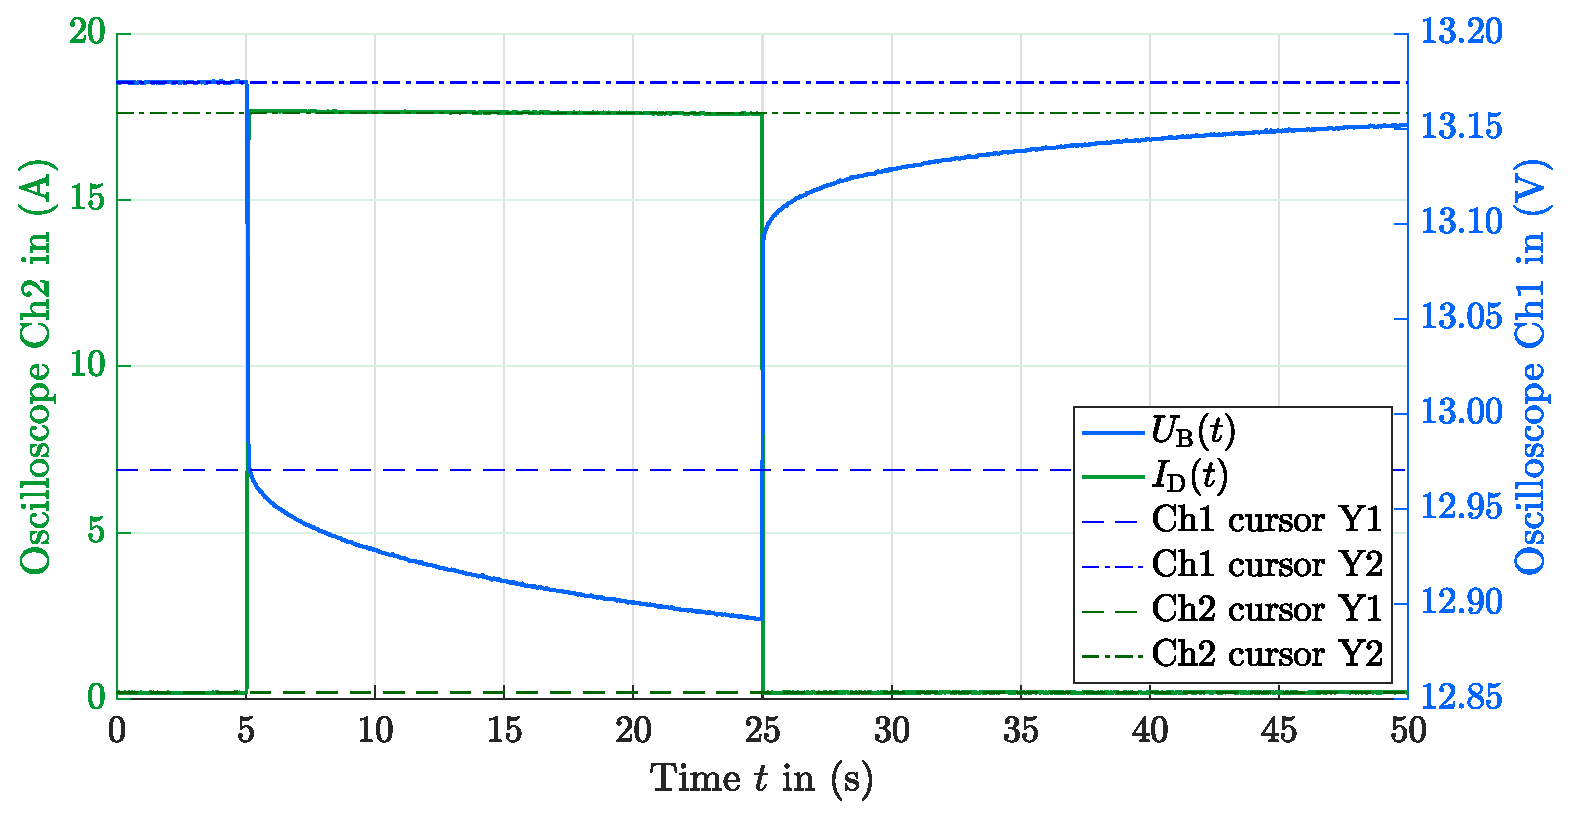
\includegraphics[width = 0.9\textwidth]{image_dis_50.eps}
  	\caption{Recorded time courses of $U_\mathrm{B}(t)$ and $I_\mathrm{D}(t)$ during the discharging experiment for $\mathrm{SOC}_n = 0,50$. The device under test was the Offgridtec Smart-Pro $12,8\mathrm{V}$ $50\mathrm{Ah}$ $\mathrm{LiFePO_4}$ battery.}
	\label{fig:image_dis_50}
\end{figure}
\begin{figure}[h!]
	\centering
  	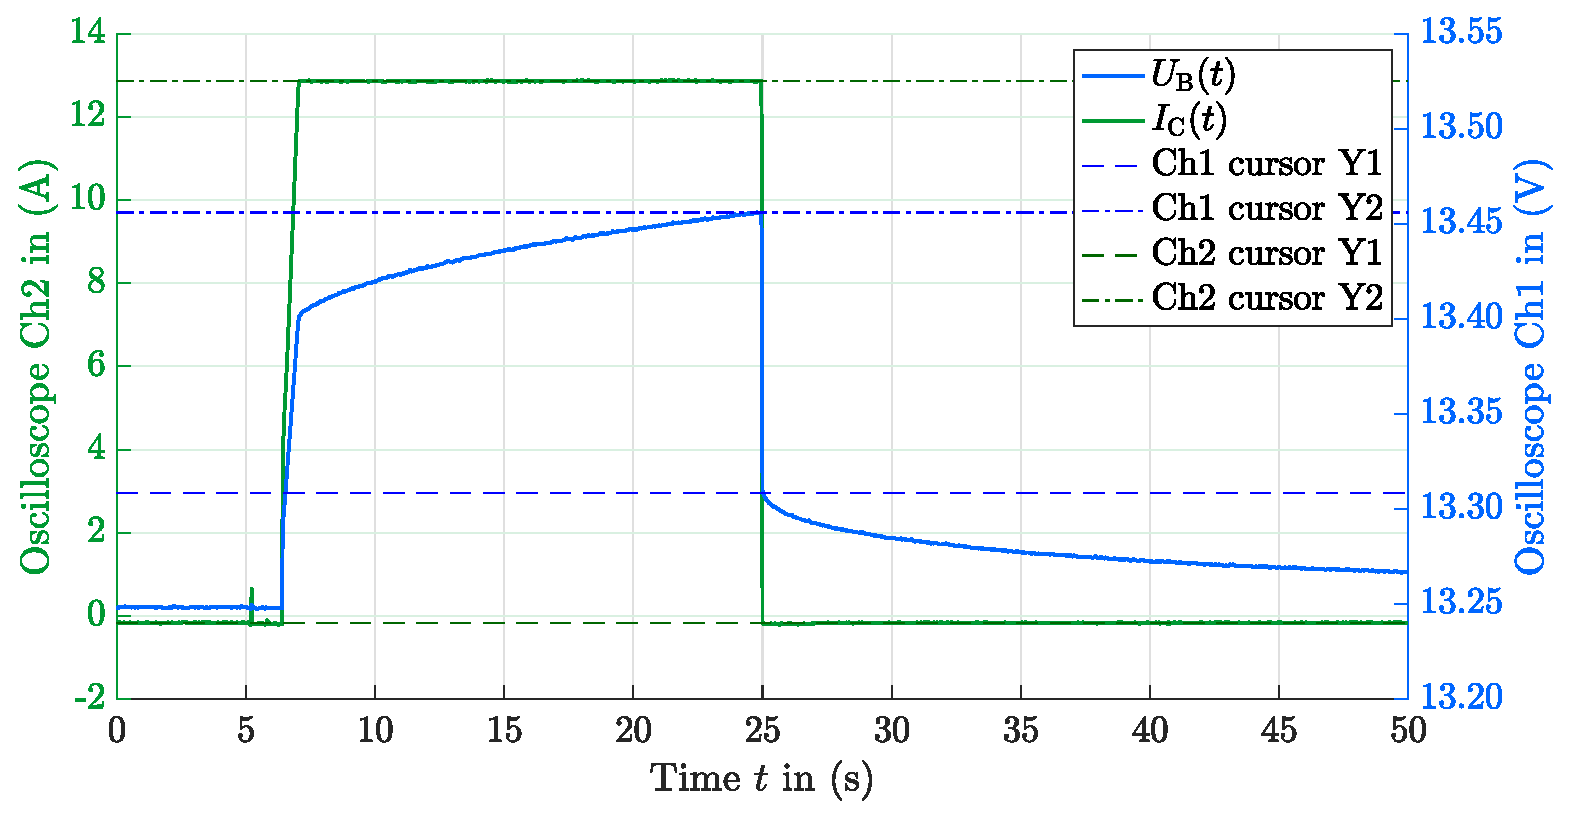
\includegraphics[width = 0.9\textwidth]{image_chg_50.eps}
	\caption{Recorded time courses of $U_\mathrm{B}(t)$ and $I_\mathrm{C}(t)$ during the charging experiment for $\mathrm{SOC}_n = 0,50$. The device under test was the Offgridtec Smart-Pro $12,8\mathrm{V}$ $50\mathrm{Ah}$ $\mathrm{LiFePO_4}$ battery.}
	\label{fig:image_chg_50}
\end{figure}

The time courses of the channels 1 and 2 shown in the figures \ref{fig:image_dis_50} and \ref{fig:image_chg_50} were recorded with the oscilloscope for all measuring points, with each being saved in a seperate\codeword{.cvs}file. Subsequently, the data in the\codeword{.cvs}files were processed with a \MATLAB program, in which the function\codeword{ischange()}was used to determine the positions of the cursors. The currents $I_\mathrm{D}(\mathrm{SOC}_n)$ and $I_\mathrm{C}(\mathrm{SOC}_n)$ as well as the voltage drops $\Delta U_\mathrm{D}(\mathrm{SOC}_n)$ and $\Delta U_\mathrm{C}(\mathrm{SOC}_n)$ were then calculated by subtracting their respective dashed cursor from their dash-dotted cursor. Now that all the required parameters were known, the electrolyte resistances $R_\mathrm{e,D}(\mathrm{SOC}_n)$ and $R_\mathrm{e,C}(\mathrm{SOC}_n)$ were determined using the equations (\ref{eq:r_0_d_soc}) and (\ref{eq:r_0_c_soc}).

For completeness it must be mentioned that the scales of the green y-axes from the figures \ref{fig:image_dis_50} and \ref{fig:image_chg_50} were calculated with this \MATLAB program by extracting the Ch2 data -- which represents the measured voltage drop across the shunt resistor -- from the\codeword{.cvs}files and applying it to the equations (\ref{eq_i_d_real}) and (\ref{eq:i_c_real}).

It should further be noted that $\Delta t_\mathrm{D}$ and $\Delta t_\mathrm{C}$ cannot be seen in the figures \ref{fig:image_dis_50} and \ref{fig:image_chg_50}, since these are the time intervals between two successive measuring points. The time interval between switching the discharging or charging current on and off -- for a certain measuring point -- was determined during the course of the experiments. When $t_\mathrm{rest}$ was over, the open-circuit voltages $U_\mathrm{0,D}(\mathrm{SOC}_n)$ and $U_\mathrm{0,C}(\mathrm{SOC}_n)$ were measured, the time scale of the oscilloscope was set to 50s and Ch1 was triggered manually. After approximately 5s, either the electronic load or the charger was switched on manually. After another 20s these were switched off again. This approach gave the best results. From the measured open-circuit voltages, $U_\mathrm{0}(\mathrm{SOC}_n)$ was calculated with the equation (\ref{eq:U_0}).

The results of the experiments are summarized in the table \ref{tab:table_exp_results} and visualized in the figures \ref{fig:image_open_circuit_voltages_matlab} and \ref{fig:image_electrolyte_resistances_matlab}. To obtain the battery model, these now only have to be interpolated and inserted into the equation (\ref{eq:battery_voltage_adapted}). 
\begin{table}[h!]
	\centering
	\footnotesize
\begin{tabular}{|c|c|c|c|c|c|}
	\hline
	$\boldsymbol{\mathrm{SOC}_n}$ & $\boldsymbol{R_\mathrm{e,D}(\mathrm{SOC}_n)}$ & $\boldsymbol{R_\mathrm{e,C}(\mathrm{SOC}_n)}$ & $\boldsymbol{U_\mathrm{0,D}(\mathrm{SOC}_n)}$ & $\boldsymbol{U_\mathrm{0,C}(\mathrm{SOC}_n)}$ & $\boldsymbol{U_\mathrm{0}(\mathrm{SOC}_n)}$ \\
	\hline
1,00 & $0,0121\Omega$ & $0,0121\Omega$ & $13,877\mathrm{V}$ & $14,107\mathrm{V}$ & $13,9920\mathrm{V}$\\ 
0,95 & $0,0117\Omega$ & $0,0113\Omega$ & $13,315\mathrm{V}$ & $13,387\mathrm{V}$ & $13,3510\mathrm{V}$\\ 
0,90 & $0,0118\Omega$ & $0,0115\Omega$ & $13,319\mathrm{V}$ & $13,393\mathrm{V}$ & $13,3560\mathrm{V}$\\ 
0,85 & $0,0117\Omega$ & $0,0114\Omega$ & $13,322\mathrm{V}$ & $13,401\mathrm{V}$ & $13,3615\mathrm{V}$\\ 
0,80 & $0,0116\Omega$ & $0,0115\Omega$ & $13,320\mathrm{V}$ & $13,415\mathrm{V}$ & $13,3675\mathrm{V}$\\ 
0,75 & $0,0116\Omega$ & $0,0116\Omega$ & $13,306\mathrm{V}$ & $13,388\mathrm{V}$ & $13,3470\mathrm{V}$\\ 
0,70 & $0,0117\Omega$ & $0,0112\Omega$ & $13,248\mathrm{V}$ & $13,387\mathrm{V}$ & $13,3175\mathrm{V}$\\ 
0,65 & $0,0116\Omega$ & $0,0112\Omega$ & $13,196\mathrm{V}$ & $13,275\mathrm{V}$ & $13,2355\mathrm{V}$\\ 
0,60 & $0,0116\Omega$ & $0,0111\Omega$ & $13,181\mathrm{V}$ & $13,272\mathrm{V}$ & $13,2265\mathrm{V}$\\ 
0,55 & $0,0117\Omega$ & $0,0112\Omega$ & $13,117\mathrm{V}$ & $13,253\mathrm{V}$ & $13,1850\mathrm{V}$\\ 
0,50 & $0,0117\Omega$ & $0,0113\Omega$ & $13,174\mathrm{V}$ & $13,250\mathrm{V}$ & $13,2120\mathrm{V}$\\ 
0,45 & $0,0117\Omega$ & $0,0113\Omega$ & $13,172\mathrm{V}$ & $13,248\mathrm{V}$ & $13,2100\mathrm{V}$\\ 
0,40 & $0,0118\Omega$ & $0,0114\Omega$ & $13,169\mathrm{V}$ & $13,250\mathrm{V}$ & $13,2095\mathrm{V}$\\ 
0,35 & $0,0118\Omega$ & $0,0115\Omega$ & $13,111\mathrm{V}$ & $13,244\mathrm{V}$ & $13,1775\mathrm{V}$\\ 
0,30 & $0,0118\Omega$ & $0,0114\Omega$ & $13,087\mathrm{V}$ & $13,225\mathrm{V}$ & $13,1560\mathrm{V}$\\ 
0,25 & $0,0118\Omega$ & $0,0115\Omega$ & $13,012\mathrm{V}$ & $13,179\mathrm{V}$ & $13,0955\mathrm{V}$\\ 
0,20 & $0,0118\Omega$ & $0,0116\Omega$ & $12,931\mathrm{V}$ & $13,089\mathrm{V}$ & $13,0100\mathrm{V}$\\ 
0,15 & $0,0118\Omega$ & $0,0115\Omega$ & $12,837\mathrm{V}$ & $12,958\mathrm{V}$ & $12,8975\mathrm{V}$\\ 
0,10 & $0,0117\Omega$ & $0,0117\Omega$ & $12,814\mathrm{V}$ & $12,923\mathrm{V}$ & $12,8685\mathrm{V}$\\ 
0,05 & $0,0118\Omega$ & $0,0118\Omega$ & $12,350\mathrm{V}$ & $12,502\mathrm{V}$ & $12,4260\mathrm{V}$\\ 
0,00 & $0,0121\Omega$ & $0,0121\Omega$ & $11,371\mathrm{V}$ & $11,420\mathrm{V}$ & $11,3955\mathrm{V}$\\
	\hline
\end{tabular}
	\caption{Calculated results from the discharging and charging experiment carried out on the Offgridtec Smart-Pro $12,8\mathrm{V}$ $50\mathrm{Ah}$ $\mathrm{LiFePO_4}$ battery.}
	\label{tab:table_exp_results}
\end{table}
\begin{figure}[h!]
	\centering
  	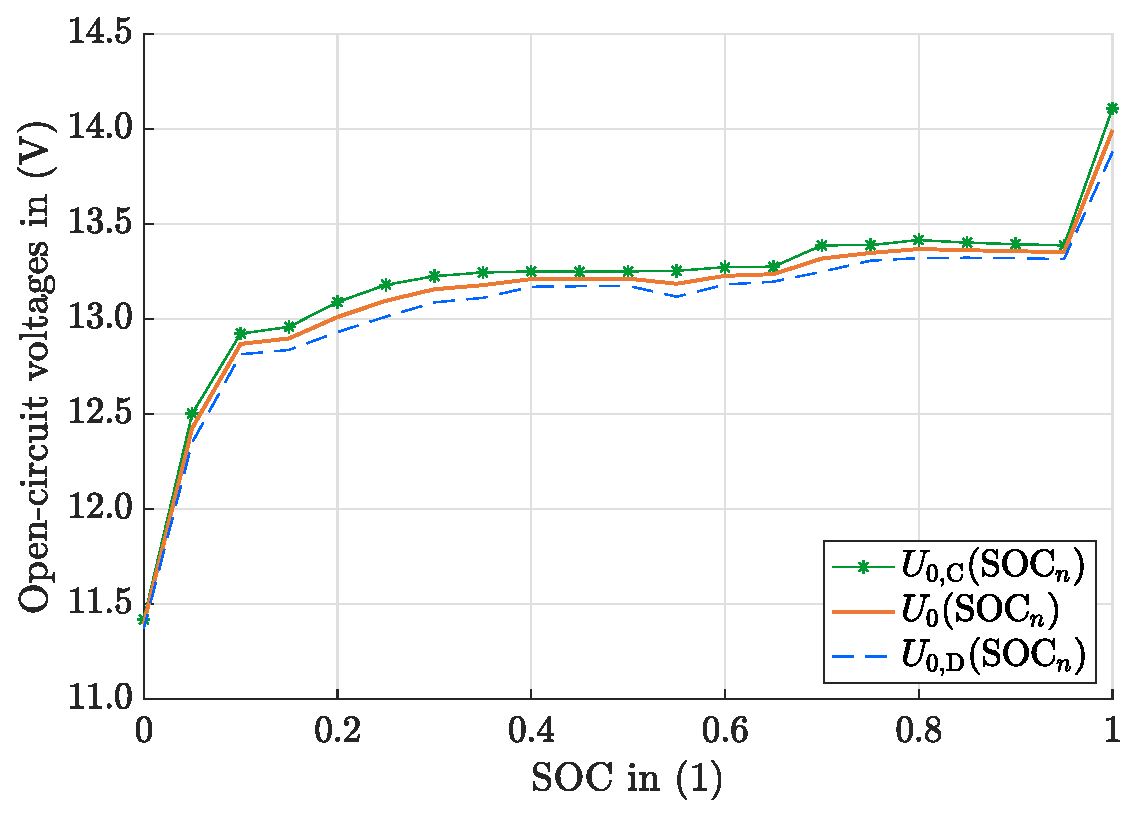
\includegraphics[width = 0.67\textwidth]{image_open_circuit_voltages_matlab.eps}
  	\caption{Open-circuit voltages $U_\mathrm{0,C}(\mathrm{SOC}_n)$, $U_\mathrm{0}(\mathrm{SOC}_n)$ and $U_\mathrm{0,D}(\mathrm{SOC}_n)$ obtained from the discharging and charging experiment carried out on the Offgridtec Smart-Pro $12,8\mathrm{V}$ $50\mathrm{Ah}$ $\mathrm{LiFePO_4}$ battery.}
	\label{fig:image_open_circuit_voltages_matlab}
\end{figure}
\begin{figure}[h!]
	\centering
  	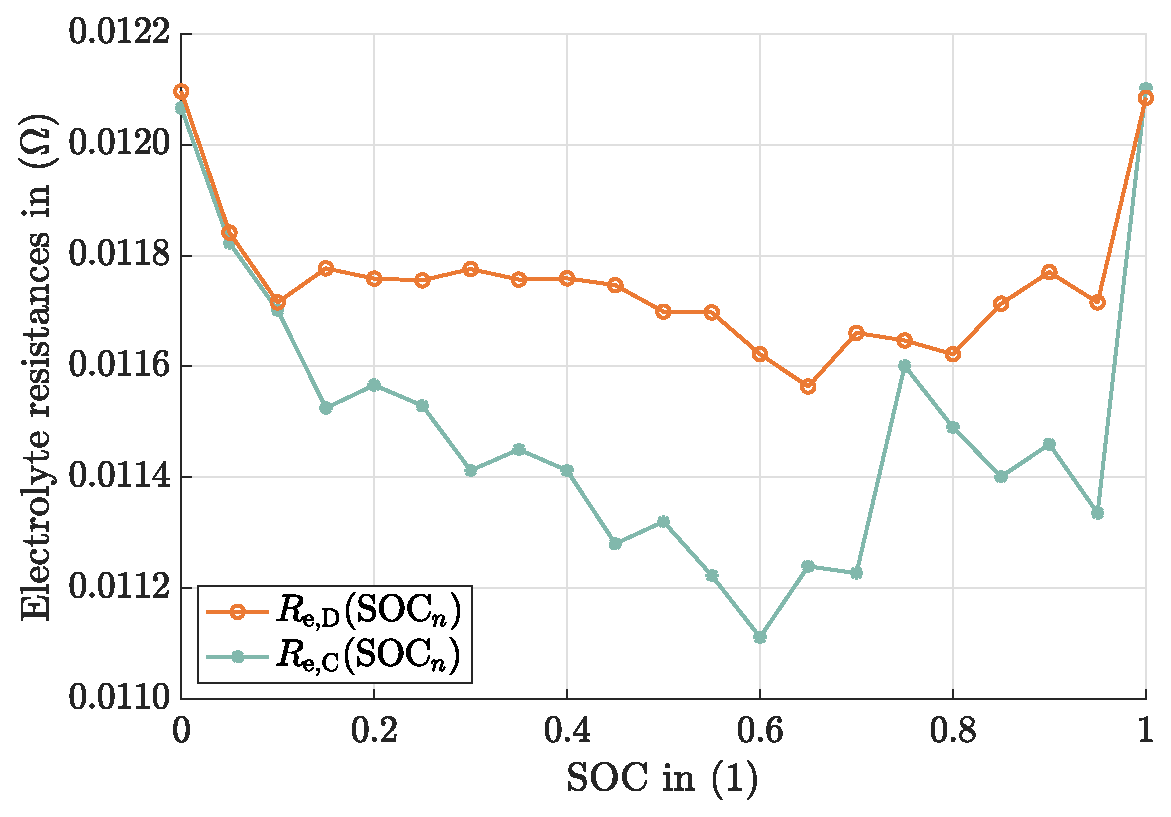
\includegraphics[width = 0.67\textwidth]{image_electrolyte_resistances_matlab.eps}
  	\caption{Electrolyte resistances $R_\mathrm{e,D}(\mathrm{SOC}_n)$ and $R_\mathrm{e,C}(\mathrm{SOC}_n)$ obtained from the discharging and charging experiment carried out on the Offgridtec Smart-Pro $12,8\mathrm{V}$ $50\mathrm{Ah}$ $\mathrm{LiFePO_4}$ battery.}
	\label{fig:image_electrolyte_resistances_matlab}
\end{figure}

Now it only remains to be shown that the assumptions for the equations (\ref{eq:battery_charge_cases}) and (\ref{current_cases}) are correct. For this purpose, the course of the charging current $I_\mathrm{C}(t)$ during the CV charging phase was measured for $\mathrm{SOC} \approx 0,99$ -- which was monitored via the Offgridtec Battery Viewer Smart app -- with Ch2 of the oscilloscope. The result can be seen in the figure \ref{fig:image_tau_b_matlab}, with the red continuous line representing the measured charging current. 
\begin{figure}[h!]
	\centering
  	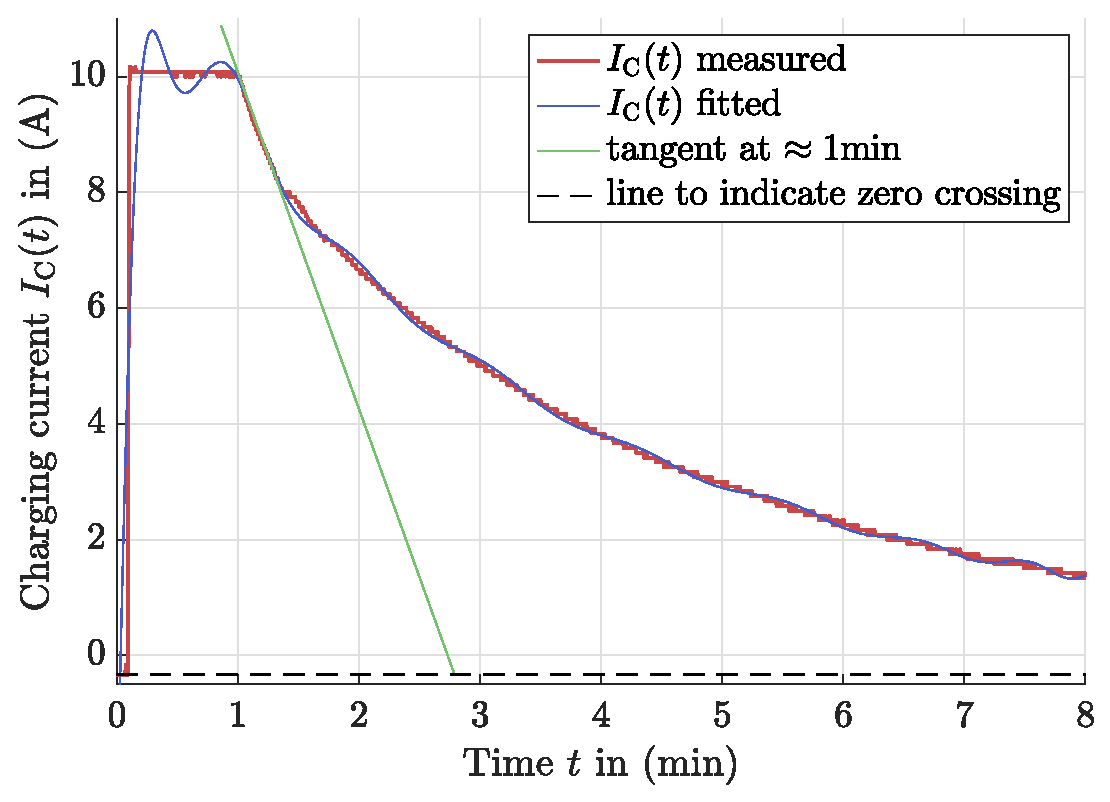
\includegraphics[width = 0.67\textwidth]{image_tau_b_matlab.eps}
  	\caption{Time course of $I_\mathrm{C}(t)$ over time during the CV charging phase of the Mean Well ENC-180-12 battery charger. The charged device was the Offgridtec Smart-Pro $12,8\mathrm{V}$ $50\mathrm{Ah}$ $\mathrm{LiFePO_4}$ battery.}
	\label{fig:image_tau_b_matlab}
\end{figure}
To prepare this measurement, the charging process of the almost fully charged battery ($\mathrm{SOC} \approx 0,99$) was switched off as soon as a decrease in the charging current was observed with Ch2 of the oscilloscope. This indicated that the battery charger was transitioning from the CC to the CV charging phase. Thereafter the battery was left to rest for 20min. The measurement was then recorded by setting the time scale of the oszilloscope to 8min, triggering Ch2 manually and continuing the charging process. First, the battery charger went into the CC charging phase and then, $t_1 = 1 \mathrm{min}$ after the start of the measurement, into the CV charging phase. No steep drop in the charging current can be seen from the recorded measurement (compare to figure \ref{fig:image_tau_b_matlab}). Thus, the described model for charging and discharging the battery from the equations (\ref{eq:battery_charge_cases}) and (\ref{current_cases}) is used for the \MATLAB simulation in the appendix \ref{sec:matlab_code}. 

As can be seen, the measured data was fitted with a polynomial function illustrated with the blue continuous line. The tangent of the polynomial fitting function, illustrated with the green continuous line, was chosen so that it runs through the point in time $t_1 = 1\mathrm{min}$ -- at which the battery charger changes from the CC to the CV charging phase. The top and bottom values of the charging current are $10,167\mathrm{A}$ and $-0,333\mathrm{A}$, with the difference between these values being the charging current in the CC charging phase $I_\mathrm{C} = 10,5\mathrm{A}$. Based on the bottom value, the black dashed line indicates the zero crossing of the measured $I_\mathrm{C}(t)$. The intersection with this line and the tangent is at $t_2 = 2,7904\mathrm{min}$. Hence, the measured time constant of the battery follows to:
\begin{equation}\label{eq:tau_battery_measured}
	\centering
	\tau_\mathrm{B} = t_2 - t_1 = 1,7904\mathrm{min}\text{.}
\end{equation}

It can be seen from the figures \ref{fig:image_dis_50}, \ref{fig:image_chg_50} and \ref{fig:image_tau_b_matlab} that the top and bottom values for the currents $I_\mathrm{D}$ and $I_\mathrm{C}$ do not quite match the values $I_\mathrm{nom}$ and $I_\mathrm{BC}$. This is likely due to the electronic loads and the battery charger. Since the behavior of these devices is only known from their data sheets, further investigations must be carried out in order to obtain more precise results. Alternatively, more professional devices that are certified for laboratory use can be used. Finally, a resistance measurement of the shunt resistor can be carried out in order to determine its exact resistance value.

\subsection{Performance estimation}
Now the results of the performance estimation of the self-sufficient energy distribution system for two different mission locations on Earth are presented. First for the Negev Desert in Israel, as the OeWF's next analog Mars field mission AMADEE-20 will take place there from October 4\textsuperscript{th} to October 31\textsuperscript{st}, 2021, and then for Vienna, Austria, from April 1\textsuperscript{st} to April 30\textsuperscript{th}, as this is the location where the assembled voice communication system will probably be tested.

Before the simulated results are presented, the SCC must first be briefly introduced. For the self-sufficient energy distribution system, the Victron Energy BlueSolar MPPT 75/10 solar charging controller is used. Its specifications are listed in the table \ref{tab:table_scc_specs}.
\begin{table}[h!]
	\centering
	\footnotesize
\begin{tabular}{|l|c|}
	\hline
	\multicolumn{2}{|c|}{\textbf{Victron BlueSolar MPPT 75/10 specifications}} \\
	\hline
	Battery voltage & $12\mathrm{V}$ \\
	Maximum battery current & $10\mathrm{A}$ \\
	Maximum PV generator power & $145\mathrm{W}$\\
	Maximum PV generator short-circuit current & $13\mathrm{A}$ \\
	Maximum load current & $15\mathrm{A}$ \\
	CV charging voltage & $14,4\mathrm{V}$ \\
	Float charge voltage & $13,8\mathrm{V}$ \\
	\hline
\end{tabular}
	\caption{Excerpt from the user manual of the Victron Energy BlueSolar MPPT 75/10 solar charging controller \cite{Victron:2021}.}
	\label{tab:table_scc_specs}
\end{table}
According to the user manual of this SCC, it only connects the PV generator when a voltage of $U_\mathrm{in,PV} > U_\mathrm{B} + 5\mathrm{V}$ is reached at its PV generator input terminal. It is noted that $U_\mathrm{in,PV}$ already takes the cable losses into account. After this condition is met, the PV generator remains connected to the battery and the load as long as the new condition $U_\mathrm{in,PV} > U_\mathrm{B} + 1\mathrm{V}$ is fulfilled. In its user manual it is also mentioned that the maximum power of the PV generator must not exceed $145\mathrm{W}$. If the power is exceeded, the SCC limits the current from said generator \cite{Victron:2021}.

The \MATLAB simulation in the appendix \ref{sec:matlab_code} is based on the user manual of the Victron BlueSolar MPPT 75/10 SCC, the results presented in the subsections \ref{sec:pv_gen_mod} and \ref{sec_bat_res} and the basics explained in the section \ref{sec:solar_energy}.

Although it was mentioned in the subsection \ref{sec:load_radio} that a step function can be implemented for the load current, this was not successful in \MATLAB. It should also be noted that the battery charging process explained in the subsection \ref{sec:electrochemical} was not implemented due to the effort involved. Instead, the equation \ref{eq:soc} was used, which models a linear increase or decrease in the SOC of the battery. 

The aim of the \MATLAB simulation is to calculate how the PV generator must be installed at the mission location so that it can maximize its daily electrical energy yield throughout the mission. Based on the daily electrical energy yield, the \MATLAB simulation calculates the SOC of the battery for each mission day. It then gives a feedback if the the battery can be fully charged during the course of the mission. If this is the case, it is likely that the repeater radio system can be supplied with enough electrical energy. However, if the battery cannot be fully charged during the course of the mission, one or more PV generators must be connected in parallel to the existing one to increase the current $I_\mathrm{MPP}$, and thus $P_\mathrm{MPP}$, of the PV generator array \cite{Mertens:2015}. For completenss it is noted that the \MATLAB simulation assumes that the PV generators connected in parallel are the same type. In addition to that, the simulation can throw several error messages if either the conditions in the equations \ref{eq:h_sunrise} and \ref{eq:h_sunset} are not met, the voltage at the repeater is too low or to high, or if the battery gets fully discharged during the course of the mission.

Based on the simulation inputs for the Negev Desert in Israel and for Vienna, Austria, in the tables \ref{tab:table_negev} and \ref{tab:table_vienna}, the command window outputs of the \MATLAB simulation result in the listings \ref{lst:list_negev_1} and \ref{lst:list_negev_2} for the Negev Desert and in the listings \ref{lst:list_negev_3} and \ref{lst:list_negev_4} for Vienna. The global horizontal irradiation, direct normal irradiation and average ambient temperature for the Negev Desert can be obtained from the figures \ref{fig:temp_negev} to \ref{fig:dni_israel} and for Vienna from the figures \ref{fig:ghi_austria}, \ref{fig:dni_austria} and \ref{fig:temp_vienna}. %% CHANGE TABLES IF NECESSARY 
\begin{table}[h!]
	\centering
	\footnotesize
\begin{tabular}{|l|c|}
	\hline
	\multicolumn{2}{|c|}{\textbf{Simulation input for the Negev Desert in Israel}} \\
	\hline
	Latitude & $30,500^\circ$ N \\
	Longitude & $34,917^\circ$ E \\ 
	Date of mission start & October 4\textsuperscript{th} 2021 \\
	Date of mission end & October 31\textsuperscript{st} 2021 \\
	Daily mission start (UTC) & 4:00h \\
	Daily mission end (UTC) & 14:00h \\
	Average ambient temperature & $22,3^\circ \mathrm{C}$ \\
	Global horizontal irradiation & $6,05\mathrm{kWhm}^{-2}$ \\
	Direct normal irradiation & $6,85\mathrm{kWhm}^{-2}$ \\
	Albedo of the ground (Sand) & $0,30$ \\
	Repeater radio system duty cycle ($a_\mathrm{T}/a_\mathrm{R}/a_\mathrm{Stby}$) & $20\%/20\%/60\%$ \\
	PV generator & AE Solar AE195SMM6-36 \\
	Number of PV generators & $1$ \\
	Initial state of charge of the battery & $0,6$ \\
	\hline
\end{tabular}
	\caption{Input for the \MATLAB simulation of the self-sufficient energy distribution system for the Negev Desert in Israel.}
	\label{tab:table_negev}
\end{table}
\begin{table}[h!]
	\centering
	\footnotesize
\begin{tabular}{|l|c|}
	\hline
	\multicolumn{2}{|c|}{\textbf{Simulation input for Vienna, Austria}} \\
	\hline
	Latitude & $48,210^\circ$ N \\
	Longitude & $16,363^\circ$ E \\ 
	Date of mission start & April 1\textsuperscript{st} 2021 \\
	Date of mission end & April 30\textsuperscript{th} 2021 \\
	Daily mission start (UTC) & 5:00h \\
	Daily mission end (UTC) & 15:00h \\
	Average ambient temperature & $11,4^\circ \mathrm{C}$ \\
	Global horizontal irradiation & $3,25\mathrm{kWhm}^{-2}$ \\
	Direct normal irradiation & $2,90\mathrm{kWhm}^{-2}$ \\
	Albedo of the ground (Grass) & $0,25$ \\
	Repeater radio system duty cycle ($a_\mathrm{T}/a_\mathrm{R}/a_\mathrm{Stby}$) & $20\%/20\%/60\%$ \\
	PV generator & AE Solar AE195SMM6-36 \\
	Number of PV generators & $2$ (parallel) \\
	Initial state of charge of the battery & $0,6$ \\
	\hline
\end{tabular}
	\caption{Input for the \MATLAB simulation of the self-sufficient energy distribution system for Vienna, Austria.}
	\label{tab:table_vienna}
\end{table}
\begin{figure}[h!]
	\centering
  	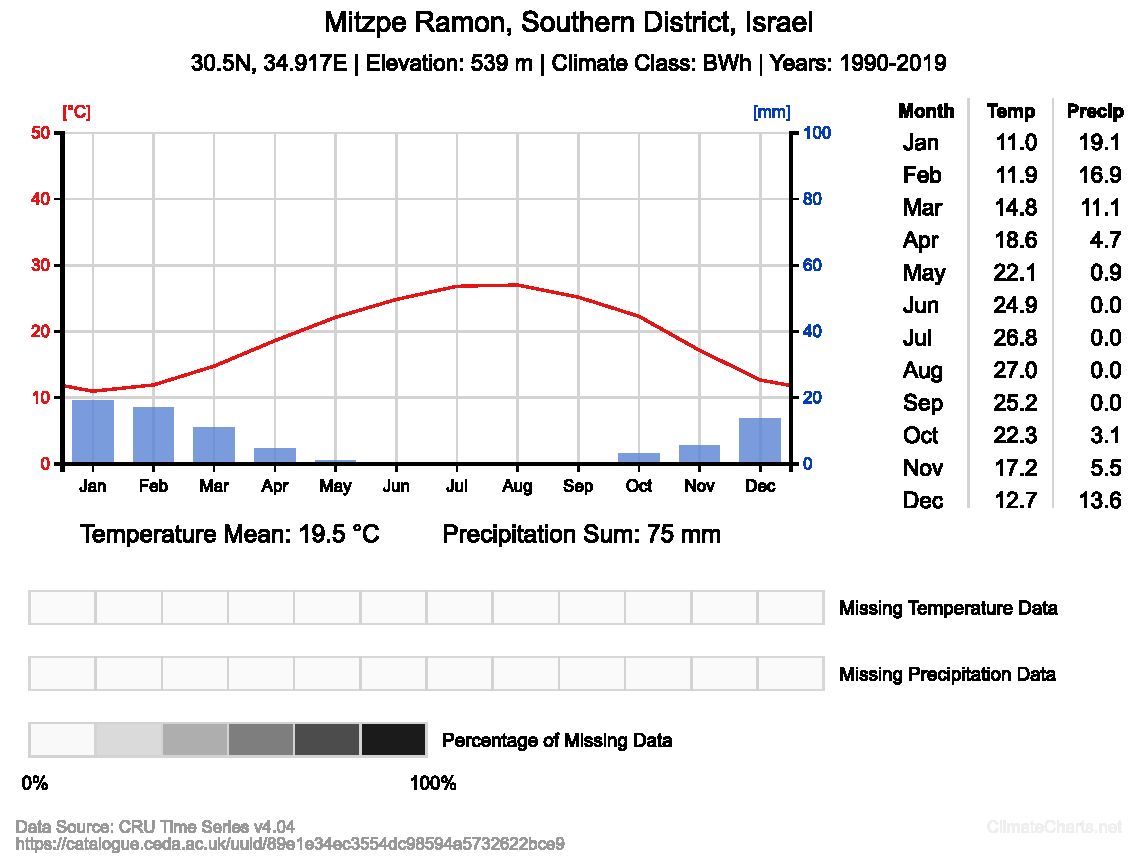
\includegraphics[width = 0.96\textwidth]{temp_maps/temp_negev}
  	\caption{Monthly averages of temperature and precipitation data for Mitzpe Ramon, Southern District, Israel (Negev Desert). (Image credit: \cite{Zepner:2020})}
	\label{fig:temp_negev}
\end{figure}

\begin{lstfloat}
\begin{lstlisting}[numbers = none, caption = {Output of the \MATLAB simulation in appendix \ref{sec:matlab_code} regarding the installation of the PV generator for the mission inputs in the table \ref{tab:table_negev}.}, label = lst:list_negev_1, captionpos = b]
              *******************************************
              [OUTPUT] PV GENERATOR INSTALLATION:

              Mission day | Opt. tilt angle | Orientation
              -------------------------------------------
              04-Oct-2021 |    35.78 deg    |    SOUTH
              05-Oct-2021 |    36.18 deg    |    SOUTH
              06-Oct-2021 |    36.57 deg    |    SOUTH
              07-Oct-2021 |    36.96 deg    |    SOUTH
              08-Oct-2021 |    37.34 deg    |    SOUTH
              09-Oct-2021 |    37.73 deg    |    SOUTH
              10-Oct-2021 |    38.11 deg    |    SOUTH
              11-Oct-2021 |    38.49 deg    |    SOUTH
              12-Oct-2021 |    38.87 deg    |    SOUTH
              13-Oct-2021 |    39.25 deg    |    SOUTH
              14-Oct-2021 |    39.62 deg    |    SOUTH
              15-Oct-2021 |    39.99 deg    |    SOUTH
              16-Oct-2021 |    40.36 deg    |    SOUTH
              17-Oct-2021 |    40.72 deg    |    SOUTH
              18-Oct-2021 |    41.08 deg    |    SOUTH
              19-Oct-2021 |    41.44 deg    |    SOUTH
              20-Oct-2021 |    41.80 deg    |    SOUTH
              21-Oct-2021 |    42.15 deg    |    SOUTH
              22-Oct-2021 |    42.50 deg    |    SOUTH
              23-Oct-2021 |    42.84 deg    |    SOUTH
              24-Oct-2021 |    43.18 deg    |    SOUTH
              25-Oct-2021 |    43.52 deg    |    SOUTH
              26-Oct-2021 |    43.86 deg    |    SOUTH
              27-Oct-2021 |    44.19 deg    |    SOUTH
              28-Oct-2021 |    44.51 deg    |    SOUTH
              29-Oct-2021 |    44.83 deg    |    SOUTH
              30-Oct-2021 |    45.15 deg    |    SOUTH
              31-Oct-2021 |    45.46 deg    |    SOUTH
              -------------------------------------------
                  Mean    |    40.80 deg    |    SOUTH

              *******************************************
\end{lstlisting}
\end{lstfloat}
Listing \ref{lst:list_negev_1} shows the optimal angle of inclination -- or tilting angle -- $\beta$ and the orientation of the normal to the PV generator's energy converting surface $A_\mathrm{PV}$, with respect to the cardinal directions, for each mission day. As explained in the subsection \ref{sec:photovoltaic_generator_alignment}, the optimal angle of inclination applies for solar noon $t_\mathrm{S} = 12\mathrm{h}$. This might not be true for cloudy days when the direct normal irradiation is weaker. During these days, $\beta$ must be reduced in order to maximize $E_\mathrm{DIFG}$ and $E_\mathrm{RGI}$ (copmare to equations \ref{eq:e_difg} and \ref{eq:e_rgi}), which causes $E_\mathrm{G}$ to increse (compare to equation \ref{eq:e_gen_ghi_dni}). Furthermore, the simulation determines the mean angle of inclination and orientation so that the PV generator only needs to be set up once at the beginning of the mission.

\begin{lstfloat}
\begin{lstlisting}[keywordstyle=\color{black}, numbers = none, caption = {Output of the \MATLAB simulation in appendix \ref{sec:matlab_code} regarding the daily energy yield of the PV generator for the mission inputs in the table \ref{tab:table_negev}.}, label = lst:list_negev_2, captionpos = b]
                 *************************************
                 [OUTPUT] PV GENERATOR ENERGY YIELD:

                 Applies for mean tilting angle and
                 orientation. The energy yield is 
                 the electrical energy yield. SOC 
                 full shows if the battery could be 
                 fully charged during the day.

                 Mission day | Energy yield | SOC full
                 -------------------------------------
                 04-Oct-2021 |   427.74 Wh  |    NO   
                 05-Oct-2021 |   428.65 Wh  |    NO   
                 06-Oct-2021 |   430.23 Wh  |    NO   
                 07-Oct-2021 |   431.09 Wh  |    NO   
                 08-Oct-2021 |   431.92 Wh  |    NO   
                 09-Oct-2021 |   433.41 Wh  |    NO   
                 10-Oct-2021 |   434.17 Wh  |   YES   
                 11-Oct-2021 |   435.61 Wh  |   YES   
                 12-Oct-2021 |   436.31 Wh  |   YES   
                 13-Oct-2021 |   437.69 Wh  |   YES   
                 14-Oct-2021 |   438.32 Wh  |   YES   
                 15-Oct-2021 |   439.64 Wh  |   YES   
                 16-Oct-2021 |   440.21 Wh  |   YES   
                 17-Oct-2021 |   441.46 Wh  |   YES   
                 18-Oct-2021 |   441.96 Wh  |   YES   
                 19-Oct-2021 |   443.15 Wh  |   YES   
                 20-Oct-2021 |   443.58 Wh  |   YES   
                 21-Oct-2021 |   444.71 Wh  |   YES   
                 22-Oct-2021 |   445.80 Wh  |   YES   
                 23-Oct-2021 |   446.12 Wh  |   YES   
                 24-Oct-2021 |   447.15 Wh  |   YES   
                 25-Oct-2021 |   447.40 Wh  |   YES   
                 26-Oct-2021 |   448.37 Wh  |   YES   
                 27-Oct-2021 |   449.30 Wh  |   YES   
                 28-Oct-2021 |   449.44 Wh  |   YES   
                 29-Oct-2021 |   450.30 Wh  |   YES   
                 30-Oct-2021 |   450.37 Wh  |   YES   
                 31-Oct-2021 |   451.16 Wh  |   YES   

                 *************************************
\end{lstlisting}
\end{lstfloat}
To display the command window output shown in the listing \ref{lst:list_negev_2}, the simulation uses the mean inclination angle from the listing \ref{lst:list_negev_1} and calculates the daily electrical energy yield of the PV generator. On the basis of this, the SOC of the battery is calculated for each mission day. An algorithm then evaluates whether the battery has been fully charged during each mission day and outputs either \codeword{YES} or \codeword{NO}. As it can be seen, the battery cannot be fully charged for the first few mission days. This is due to the assumption that the battery is $60\%$ charged at the beginning of the mission -- hence $\mathrm{SOC_{init}} = 0,6$. With this SOC, the Offgridtec Smart-Pro $12,8\mathrm{V}$ $50\mathrm{Ah}$ $\mathrm{LiFePO}_4$ battery is stored for longer periods of time \cite{Offgridtec:2020}. Therefore it can be said that the self-sufficient energy distribution system can supply the repeater radio system during the course of the analog Mars field mission AMADEE-20.

An interesting case occurs when the battery cannot be fully charged towards the end of the mission. This can happen, for instance, when the available solar energy is decreasing every day. Such results can be explained by changing seasons. In this case PV generators must be connected in parallel to guarantee sufficient electrical energy supply of the repeater radio system throughout the mission.

\begin{lstfloat}
\begin{lstlisting}[numbers = none, caption = {Output of the \MATLAB simulation in appendix \ref{sec:matlab_code} regarding the installation of the PV generator for the mission inputs in the table \ref{tab:table_vienna}.}, label = lst:list_negev_3, captionpos = b]
              *******************************************
              [OUTPUT] PV GENERATOR INSTALLATION:

              Mission day | Opt. tilt angle | Orientation
              -------------------------------------------
              01-Apr-2021 |    43.84 deg    |    SOUTH
              02-Apr-2021 |    43.44 deg    |    SOUTH
              03-Apr-2021 |    43.05 deg    |    SOUTH
              04-Apr-2021 |    42.65 deg    |    SOUTH
              05-Apr-2021 |    42.26 deg    |    SOUTH
              06-Apr-2021 |    41.87 deg    |    SOUTH
              07-Apr-2021 |    41.48 deg    |    SOUTH
              08-Apr-2021 |    41.10 deg    |    SOUTH
              09-Apr-2021 |    40.71 deg    |    SOUTH
              10-Apr-2021 |    40.33 deg    |    SOUTH
              11-Apr-2021 |    39.95 deg    |    SOUTH
              12-Apr-2021 |    39.58 deg    |    SOUTH
              13-Apr-2021 |    39.20 deg    |    SOUTH
              14-Apr-2021 |    38.83 deg    |    SOUTH
              15-Apr-2021 |    38.46 deg    |    SOUTH
              16-Apr-2021 |    38.10 deg    |    SOUTH
              17-Apr-2021 |    37.74 deg    |    SOUTH
              18-Apr-2021 |    37.38 deg    |    SOUTH
              19-Apr-2021 |    37.02 deg    |    SOUTH
              20-Apr-2021 |    36.67 deg    |    SOUTH
              21-Apr-2021 |    36.32 deg    |    SOUTH
              22-Apr-2021 |    35.97 deg    |    SOUTH
              23-Apr-2021 |    35.63 deg    |    SOUTH
              24-Apr-2021 |    35.29 deg    |    SOUTH
              25-Apr-2021 |    34.95 deg    |    SOUTH
              26-Apr-2021 |    34.62 deg    |    SOUTH
              27-Apr-2021 |    34.30 deg    |    SOUTH
              28-Apr-2021 |    33.97 deg    |    SOUTH
              29-Apr-2021 |    33.65 deg    |    SOUTH
              30-Apr-2021 |    33.34 deg    |    SOUTH
              -------------------------------------------
                  Mean    |    38.39 deg    |    SOUTH

              *******************************************
\end{lstlisting}
\end{lstfloat}
\begin{lstfloat}
\begin{lstlisting}[keywordstyle=\color{black}, numbers = none, caption = {Output of the \MATLAB simulation in appendix \ref{sec:matlab_code} regarding the daily energy yield of the PV generator for the mission inputs in the table \ref{tab:table_vienna}.}, label = lst:list_negev_4, captionpos = b]
                 *************************************
                 [OUTPUT] PV GENERATOR ENERGY YIELD:

                 Applies for mean tilting angle and
                 orientation. The energy yield is 
                 the electrical energy yield. SOC
                 full shows if the battery could be
                 fully charged during the day.

                 Mission day | Energy yield | SOC full
                 -------------------------------------
                 01-Apr-2021 |   490.62 Wh  |    NO   
                 02-Apr-2021 |   490.80 Wh  |    NO   
                 03-Apr-2021 |   490.98 Wh  |   YES   
                 04-Apr-2021 |   491.15 Wh  |   YES   
                 05-Apr-2021 |   491.31 Wh  |   YES   
                 06-Apr-2021 |   491.47 Wh  |   YES   
                 07-Apr-2021 |   491.62 Wh  |   YES   
                 08-Apr-2021 |   491.78 Wh  |   YES   
                 09-Apr-2021 |   491.93 Wh  |   YES   
                 10-Apr-2021 |   492.08 Wh  |   YES   
                 11-Apr-2021 |   492.23 Wh  |   YES   
                 12-Apr-2021 |   492.38 Wh  |   YES   
                 13-Apr-2021 |   492.53 Wh  |   YES   
                 14-Apr-2021 |   491.98 Wh  |   YES   
                 15-Apr-2021 |   492.16 Wh  |   YES   
                 16-Apr-2021 |   492.32 Wh  |   YES   
                 17-Apr-2021 |   492.48 Wh  |   YES   
                 18-Apr-2021 |   492.65 Wh  |   YES   
                 19-Apr-2021 |   492.83 Wh  |   YES   
                 20-Apr-2021 |   493.01 Wh  |   YES   
                 21-Apr-2021 |   492.51 Wh  |   YES   
                 22-Apr-2021 |   492.73 Wh  |   YES   
                 23-Apr-2021 |   492.94 Wh  |   YES   
                 24-Apr-2021 |   493.16 Wh  |   YES   
                 25-Apr-2021 |   492.70 Wh  |   YES   
                 26-Apr-2021 |   492.94 Wh  |   YES   
                 27-Apr-2021 |   493.23 Wh  |   YES   
                 28-Apr-2021 |   492.80 Wh  |   YES   
                 29-Apr-2021 |   493.09 Wh  |   YES   
                 30-Apr-2021 |   493.40 Wh  |   YES   

                 *************************************
\end{lstlisting}
\end{lstfloat}
A similar command window output can be obtained from the listings \ref{lst:list_negev_3} and \ref{lst:list_negev_4} for Vienna. Here, however, two PV generators connected in parallel are required. Besides that, simulations have shown, that the daily electrical energy yield is incresed when the angle of inlcination $\beta = 0^\circ$. This can also be recognized by analyzing the solar resources maps in the figures \ref{fig:ghi_austria} and \ref{fig:dni_austria}, because the global horizontal irradiation is greater than the direct normal irradiation. The author of the book \cite{Mertens:2015} mentions this as well. Such a simulation result can further be explained by the fact that these solar resource maps provide average values that have been recorded over several years and are therefore mainly used for the long-term planning of a PV generator array.

In order to obtain more intuitive simulation results, the SOC of the battery can be plotted over the entire duration of the mission or for individual mission days. Since the \MATLAB simulation only serves as a reference point, the on-site support crew still has to make regular checks of the battery's SOC during the mission in order to collect empirical data. Finally, it should be noted that the simulation could not provide any results for the DAS Energy DAS145PF PV generator, as it could not meet the condition $U_\mathrm{in,PV} > U_\mathrm{B} + 5\mathrm{V}$ with the solar resource maps mentioned. However, this could be different with the solar resource maps from \cite{Union:2020}. 

\begin{figure}[h!]
	\centering
  	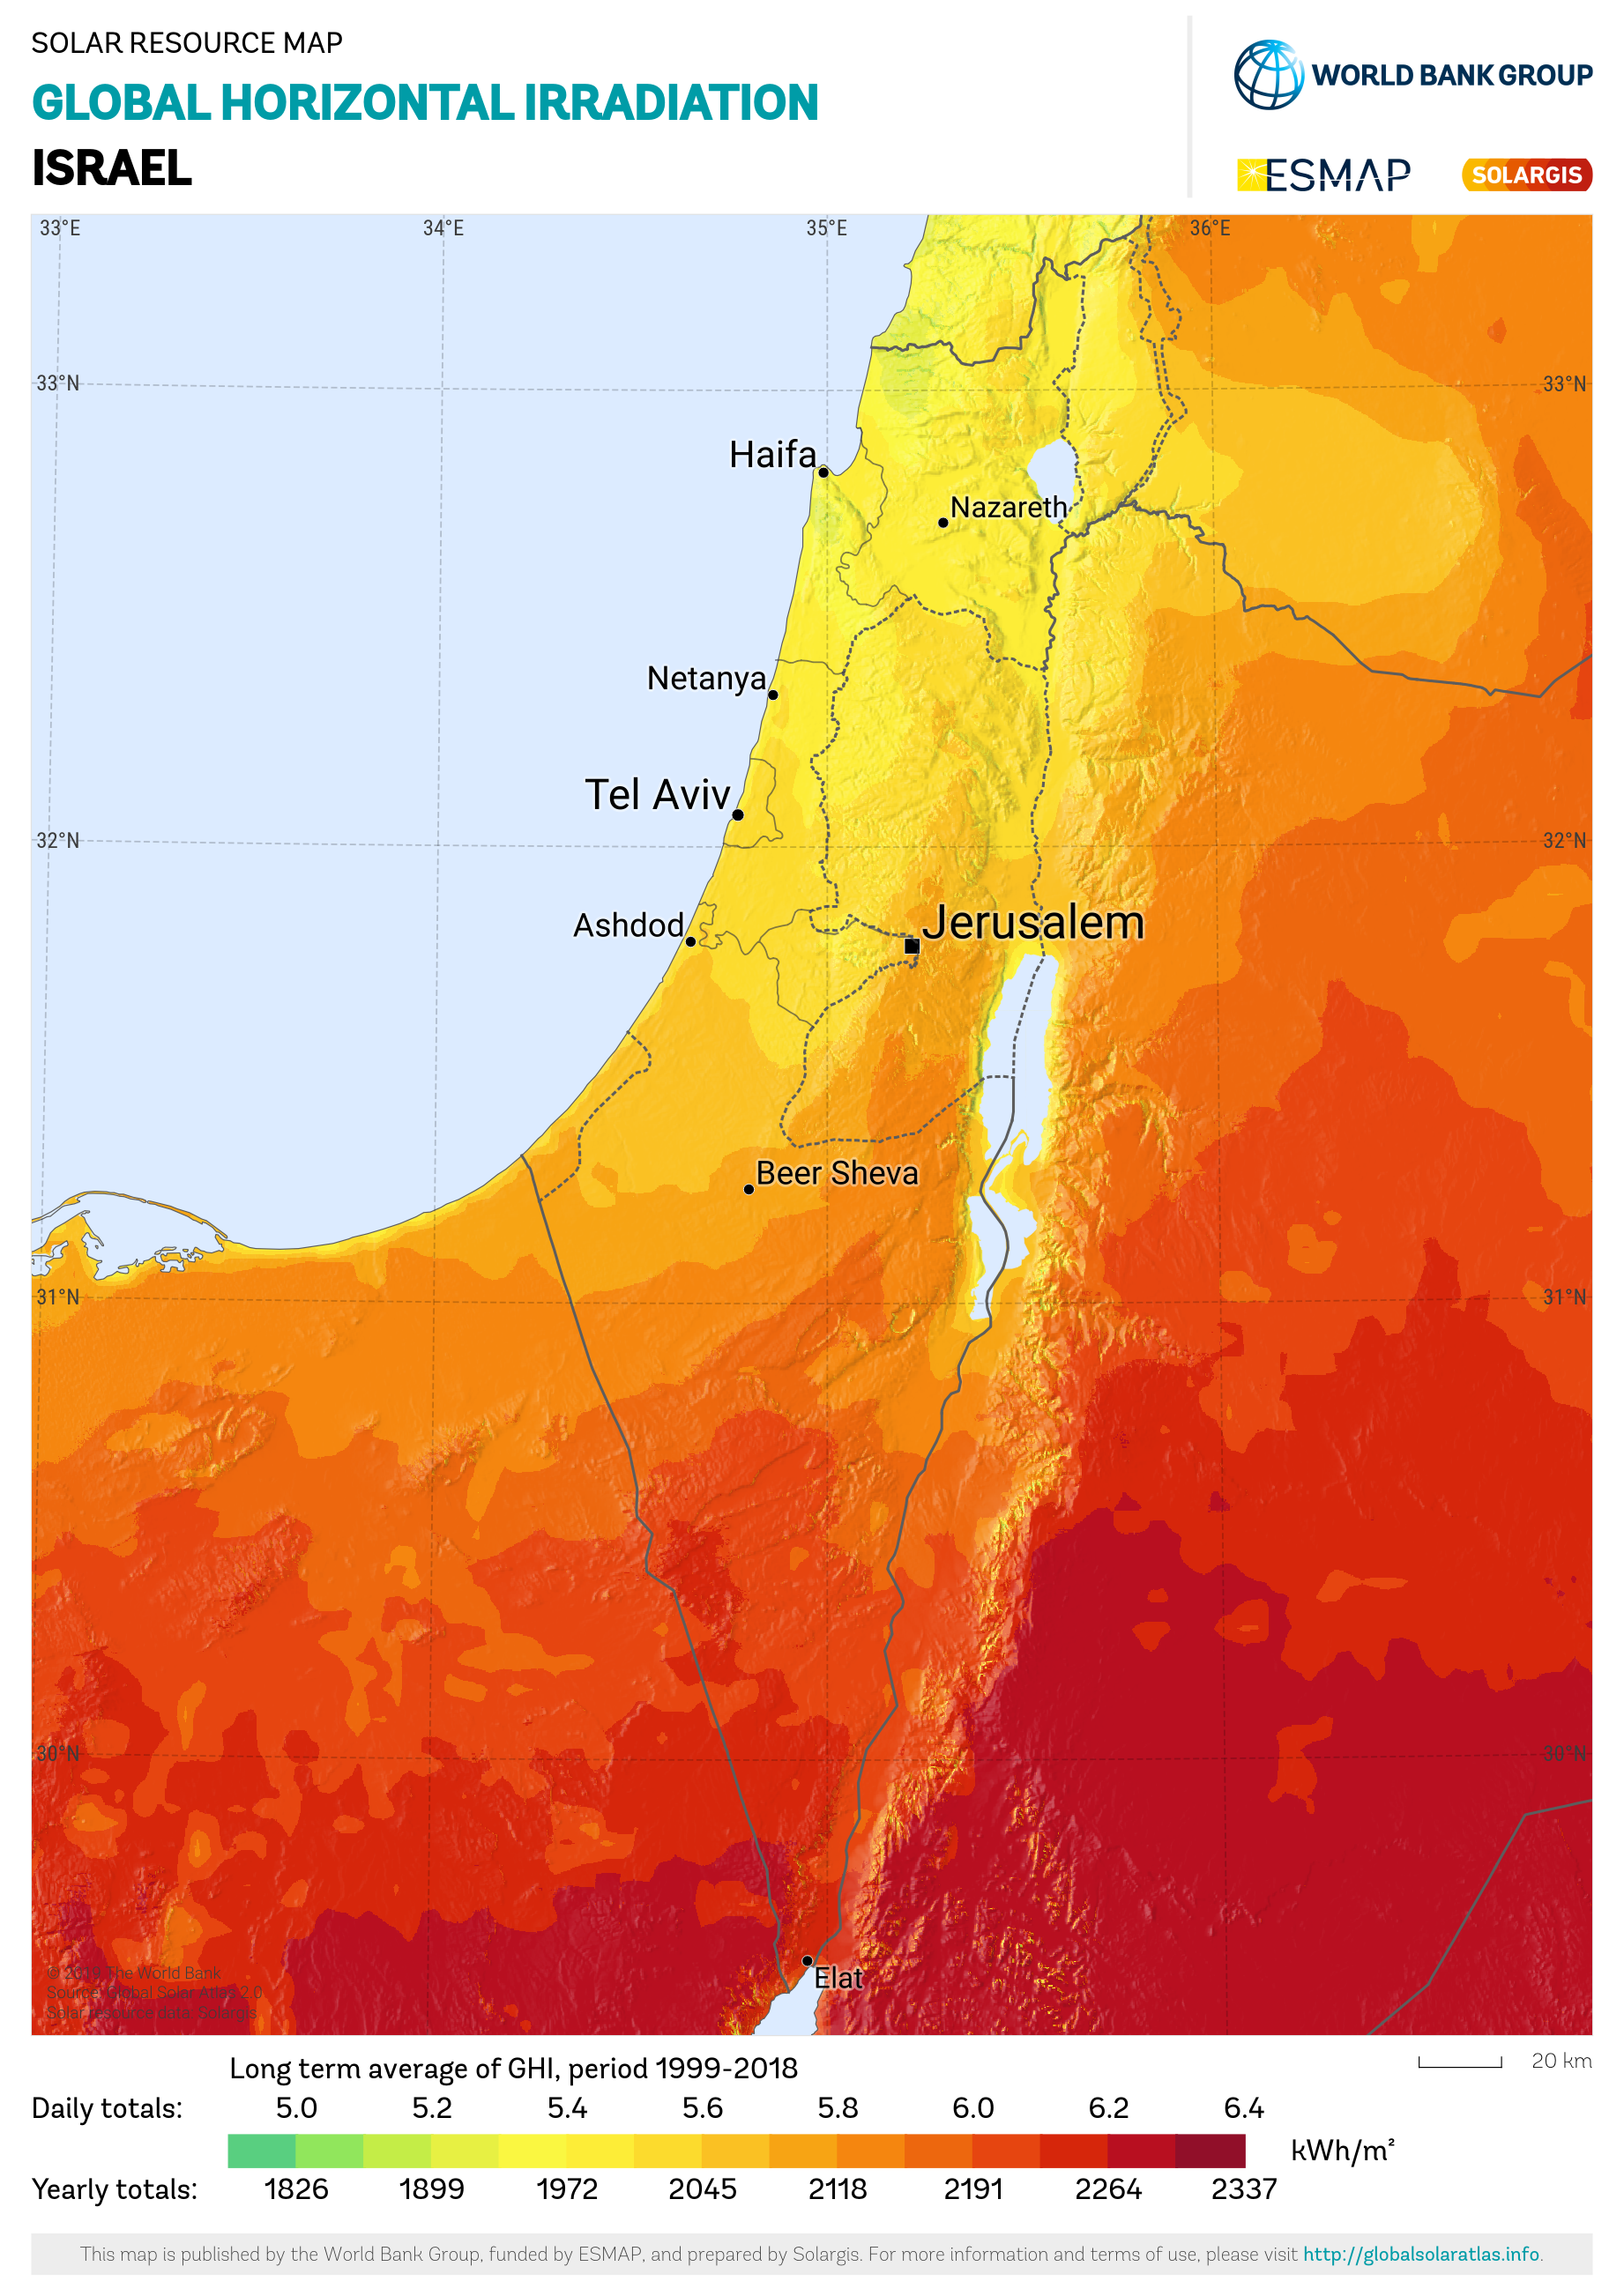
\includegraphics[width = \textwidth]{solar_maps/israel/israel_ghi}
  	\caption{Solar resource map of the long term average global horizontal irradiation of Israel. (Image credit: \cite{GlobalSolarAtlas:2020, Solargis:2021})}
	\label{fig:ghi_israel}
\end{figure}
\begin{figure}[h!]
	\centering
  	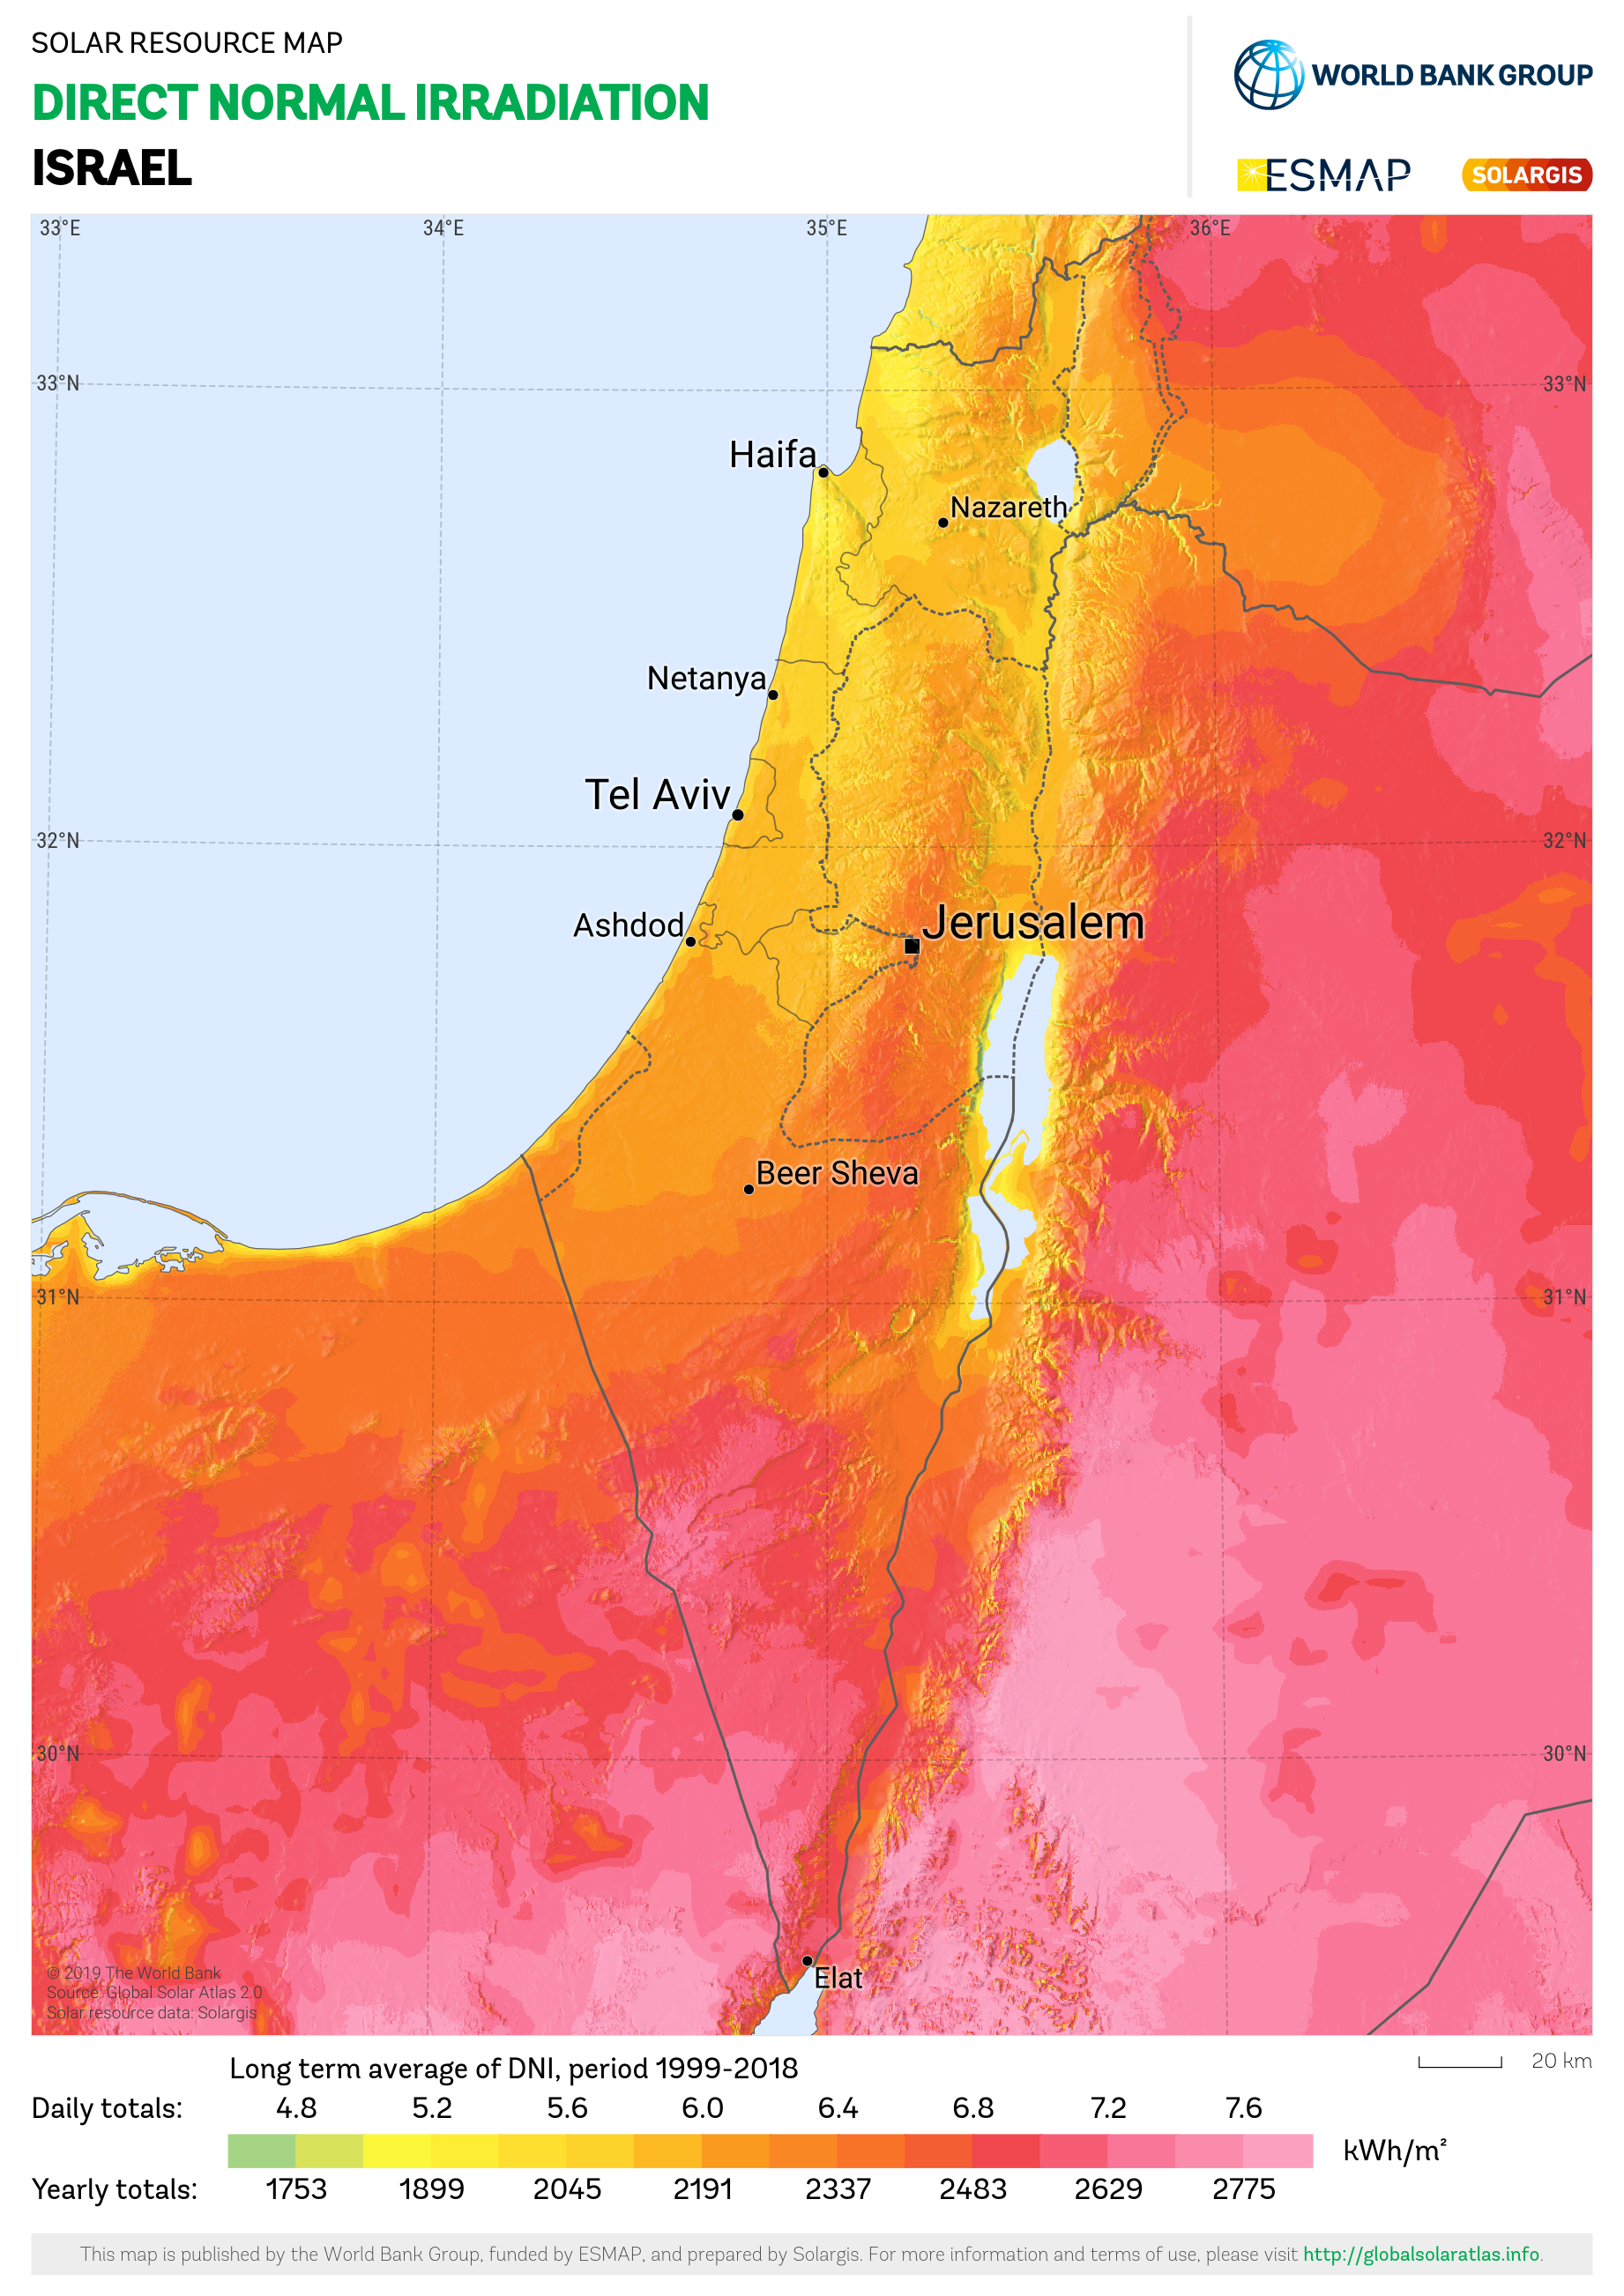
\includegraphics[width = \textwidth]{solar_maps/israel/israel_dni}
	\caption{Solar resource map of the long term average direct normal irradiation of Israel. (Image credit: \cite{GlobalSolarAtlas:2020, Solargis:2021})}
	\label{fig:dni_israel}
\end{figure}








% Warum wurde DAS Energy nicht verwendet!


% REFLECTION MAKE THE SIM BETTER AND MORE ACCURATE!!

